
\documentclass[aspectratio=1610,english]{beamer}

\usepackage{babel}
\usepackage[T1]{fontenc}
\usepackage[utf8]{inputenc}
\usepackage{lmodern}
\usepackage{amsmath,amssymb,bm}
\usepackage{booktabs}
\usepackage{graphicx}
\usepackage{array}
\usepackage{ragged2e}
\usepackage{etoolbox}
\usepackage{tikz}

\usepackage{comment}

\usetikzlibrary{calc,positioning,arrows.meta,decorations.pathmorphing,patterns}

\usepackage{hyperref}

\makeatletter
\patchcmd{\itemize}{\raggedright}{\justifying}{}{}
\patchcmd{\beamer@enum@}{\raggedright}{\justifying}{}{}
\patchcmd{\@@description}{\raggedright}{\justifying}{}{}
\makeatother

\mode<beamer>{
    \definecolor{links}{HTML}{2A1B81}
    \hypersetup{pdfpagemode=FullScreen,colorlinks,linkcolor=,urlcolor=links}
 \usetheme[parttitle=rightfooter]{AGH}
}


\graphicspath{{./}{plots_LHeC_SM_vs_BSM_delta_aTau_0p008/}{plots_LHmuC_SM_vs_BSM_delta_aTau_0p008/}}


\definecolor{TauBlue}{RGB}{25,60,180}
\definecolor{TauGreen}{RGB}{0,120,60}
\definecolor{TauOrange}{RGB}{210,110,20}
\definecolor{TauMagenta}{RGB}{210,30,220}
\definecolor{TauRed}{RGB}{180,25,40}

\newcommand{\atau}{\ensuremath{\textcolor{TauBlue}{a_{\tau}}}}
\newcommand{\datau}{\ensuremath{\textcolor{TauBlue}{\delta a_{\tau}}}}
\newcommand{\dtau}{\ensuremath{\textcolor{TauGreen}{d_{\tau}}}}
\newcommand{\ddtau}{\ensuremath{\textcolor{TauGreen}{\delta d_{\tau}}}}
\newcommand{\ctb}{\ensuremath{\textcolor{TauOrange}{C_{\tau B}}}}
\newcommand{\ctw}{\ensuremath{\textcolor{TauOrange}{C_{\tau W}}}}
\newcommand{\ctg}{\ensuremath{\textcolor{TauOrange}{C_{\tau\gamma}}}}
\newcommand{\Lam}{\ensuremath{\textcolor{TauOrange}{\Lambda}}}
\newcommand{\Mtt}{\ensuremath{M_{\tau^+\tau^-}}}
\newcommand{\Ytt}{\ensuremath{Y_{\tau^+\tau^-}}}
\newcommand{\bsmsm}{\left(\frac{d\sigma/dM}{d\sigma/dM}\right)_{\!\mathrm{BSM/SM}}}


\newcommand{\takehome}[1]{%
\begin{alertblock}{Take-home message}
\small #1
\end{alertblock}}


\newcommand{\placeholdergraphic}[2]{%
\begin{center}
\fbox{\parbox[c][#2][c]{0.86\textwidth}{\centering\vspace{1ex}\textbf{Placeholder for later screenshot}\\[0.6ex]\small #1\vspace{1ex}}}
\end{center}}


\tikzset{
    beamline/.style={line width=1.6pt,-{Latex[length=3mm,width=2.5mm]}},
    tautrack/.style={line width=1.4pt,-{Latex[length=3mm,width=2.5mm]},TauGreen},
    photon/.style={decorate,decoration={snake,amplitude=1.0mm,segment length=4mm},line width=1.0pt},
    blob/.style={circle,draw=black,fill=black,minimum size=5.5mm,inner sep=0pt},
    hatchblob/.style={circle,draw=black,pattern=north east lines,pattern color=black,minimum size=6mm,inner sep=0pt}
}

\title[Anomalous $\tau$ moments at the {\color{black}LHeC} and {\color{black}LH$\mu$C}]{Anomalous electromagnetic moments of the tau lepton\\at the {\color{black}LHeC} and {\color{black}LH$\mu$C}}
\subtitle{\small Photon-induced $\gamma\gamma\to\tau^+\tau^-$ production}
%, EFT interpretation, and truth-level sensitivity comparison}
\author[Hamzeh Khanpour]{Hamzeh Khanpour \\  % \inst{1}
{\scriptsize \href{mailto:hamzeh.khanpour@fis.agh.edu.pl}{hamzeh.khanpour@cern.ch}}}
\institute[AGH]{Faculty of Physics and Applied Computer Science\\
AGH University of Krakow
}  % \inst{1}


\date{\today}


\begin{document}

\begin{frame}[plain]
\begin{tikzpicture}[remember picture,overlay]
\node[anchor=north east, xshift=-0.60cm, yshift=-1.50cm]
at (current page.north east)
{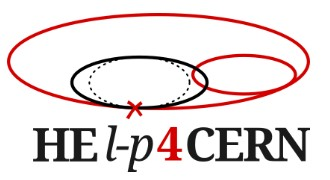
\includegraphics[width=2.5cm]{HELP4CERN.jpg}};
\end{tikzpicture}
\titlepage
\end{frame}

	
\begin{frame}{Outline}
\tableofcontents
\end{frame}




\section{Motivation and Current Status}

%=====================================================
\begin{frame}{Why anomalous electromagnetic moments of the $\tau$ lepton?}
\begin{itemize}
\justifying
\item For any charged lepton, the gyromagnetic factor is written as
    \[
      g_{\ell}=2\left(1+a_{\ell}\right),\qquad a_{\ell}=\frac{g_{\ell}-2}{2}.
    \]
\item The electron anomalous magnetic moment is measured with extraordinary precision, while the muon sector remains a long-standing arena for precision tests of quantum corrections and possible new physics.
\item The $\tau$ lepton is much heavier and experimentally less constrained; if beyond-the-Standard-Model effects scale with lepton mass, the $\tau$ sector can be especially sensitive.
\item Photon-induced $\gamma\gamma\to\tau^+\tau^-$ production provides a direct probe of the $\gamma\tau\tau$ vertex and therefore of \atau\ and \dtau.
\end{itemize}
\begin{block}{Physics target of this talk}
\small Compare the truth-level sensitivity of the {\color{red}{LHeC}} and the {\color{blue}{LH$\mu$C}} to anomalous $\tau$ electromagnetic moments using a benchmark \(\datau=0.008\) in photon-induced $\tau$-pair production.
\end{block}
\end{frame}
%=====================================================



\begin{comment}

\begin{frame}

\titlegraphic{%
	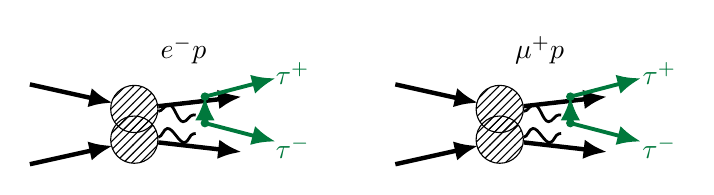
\begin{tikzpicture}[scale=0.78]
		% ep mini-diagram
		\node at (-3.1,2.0) {$e^{-}p$};
		\draw[beamline] (-5.6,1.45) -- (-4.25,1.15);
		\draw[beamline] (-5.6,0.15) -- (-4.25,0.45);
		\node[hatchblob] (epup) at (-3.9,1.05) {};
		\node[hatchblob] (epdn) at (-3.9,0.55) {};
		\draw[beamline] (epup) -- (-2.15,1.25);
		\draw[beamline] (epdn) -- (-2.15,0.35);
		\draw[photon] (epup) -- (-2.9,0.95);
		\draw[photon] (epdn) -- (-2.9,0.65);
		\fill[TauGreen] (-2.75,0.82) circle (0.07);
		\fill[TauGreen] (-2.75,1.25) circle (0.07);
		\draw[tautrack] (-2.75,0.82) -- (-2.75,1.25);
		\draw[tautrack] (-2.75,1.25) -- (-1.6,1.55);
		\draw[tautrack] (-2.75,0.82) -- (-1.6,0.52);
		\node[TauGreen] at (-1.32,1.62) {$\tau^+$};
		\node[TauGreen] at (-1.32,0.43) {$\tau^-$};
		% mup mini-diagram
		\node at (2.7,2.0) {$\mu^{+}p$};
		\draw[beamline] (0.35,1.45) -- (1.7,1.15);
		\draw[beamline] (0.35,0.15) -- (1.7,0.45);
		\node[hatchblob] (mupup) at (2.05,1.05) {};
		\node[hatchblob] (mupdn) at (2.05,0.55) {};
		\draw[beamline] (mupup) -- (3.8,1.25);
		\draw[beamline] (mupdn) -- (3.8,0.35);
		\draw[photon] (mupup) -- (3.05,0.95);
		\draw[photon] (mupdn) -- (3.05,0.65);
		\fill[TauGreen] (3.2,0.82) circle (0.07);
		\fill[TauGreen] (3.2,1.25) circle (0.07);
		\draw[tautrack] (3.2,0.82) -- (3.2,1.25);
		\draw[tautrack] (3.2,1.25) -- (4.35,1.55);
		\draw[tautrack] (3.2,0.82) -- (4.35,0.52);
		\node[TauGreen] at (4.65,1.62) {$\tau^+$};
		\node[TauGreen] at (4.65,0.43) {$\tau^-$};
\end{tikzpicture}}

\end{frame}

\end{comment}




%=====================================================
\begin{frame}{Current experimental status of $a_{\tau}$}
\begin{columns}[T]
\begin{column}{0.65\textwidth}
\begin{itemize}
\justifying
\small
\item Earlier direct constraints came from OPAL, L3, and DELPHI in the LEP era.
\item Heavy-ion measurements by ATLAS Pb+Pb and CMS Pb+Pb extended the reach using photon-induced processes at low di-$\tau$ masses.
\item The recent CMS pp analysis observed $\gamma\gamma\to\tau^+\tau^-$ and set significantly improved limits on \atau\ and \dtau [{\color{blue}Rept. Prog. Phys. 87 (2024) 107801}].
\item The present future-collider study is motivated by the same central idea: {\color{red}the BSM effect becomes more visible in the hard region of the mass spectrum.}
\end{itemize}
\begin{exampleblock}{Representative CMS pp context}
\justifying
\small Observed significance \(\sim 5.3\sigma\); 95\% CL interval roughly \(-0.0042<\atau<0.0062\); complementary constraints also obtained on \dtau.
\end{exampleblock}
\end{column}

\begin{column}{0.45\textwidth}
\begin{figure}
\centering
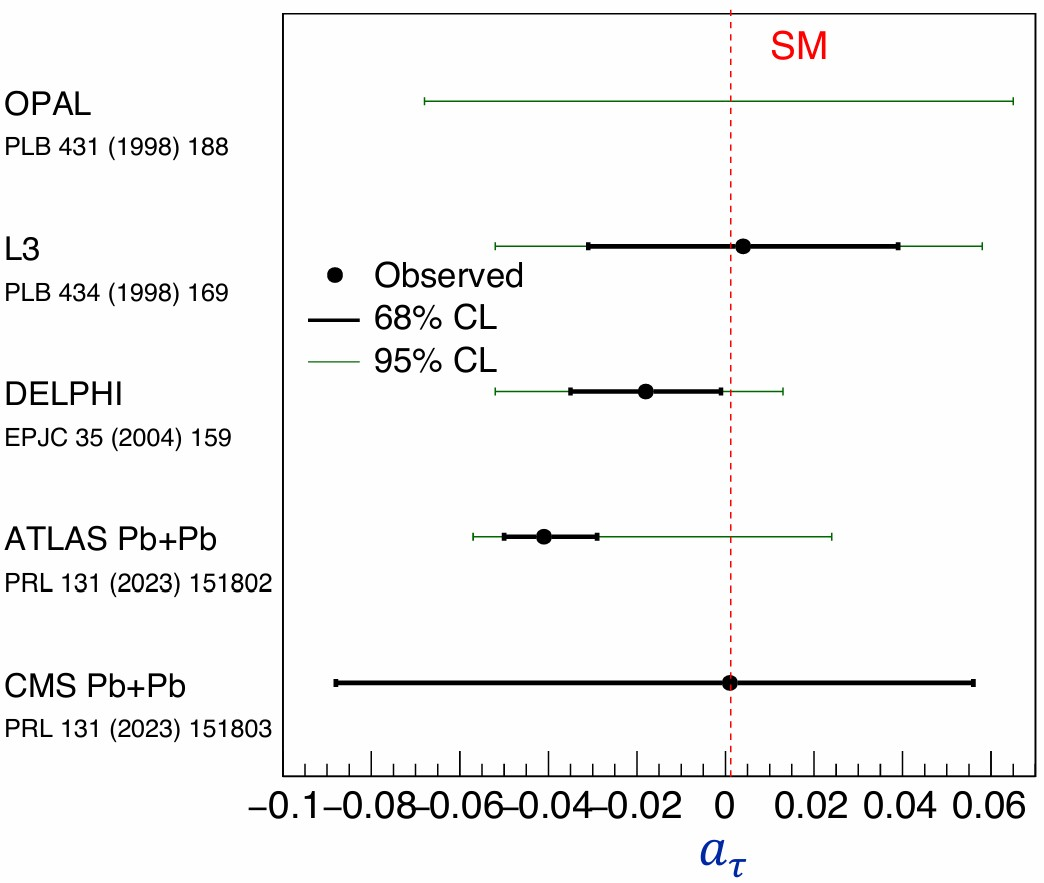
\includegraphics[width=\linewidth]{cms_world_aTau_dTau.jpg}
\caption{\small \justifying
World-comparison plot for the anomalous tau magnetic moment \(\atau\) and electric dipole moment \(\dtau\), including LEP, heavy-ion, and CMS \(pp\) constraints. }
\end{figure}
\end{column}

\end{columns}
\end{frame}
%=====================================================



%=====================================================
\begin{frame}{Why photon-induced $\gamma\gamma\to\tau^+\tau^-$?}
\begin{columns}[T]
\begin{column}{0.65\textwidth}
\begin{itemize}
 \justifying
\small
\item The process probes the \(\gamma\tau\tau\) interaction directly and cleanly.
\item In hadron or lepton--hadron environments, equivalent-photon emission from the beams can produce a relatively simple electromagnetic initial state.
\item The invariant-mass spectrum of the $\tau^+\tau^-$ pair is particularly powerful because {\color{blue}anomalous dipole-type couplings harden the high-mass tail}.
\item This makes the process attractive both for present measurements and for future-machine sensitivity studies.
\end{itemize}
\takehome{
 \justifying \small The most important discriminating observable is the hard tail of the \(\tau^+\tau^-\) invariant-mass distribution.}
\end{column}

\begin{column}{0.45\textwidth}
\begin{figure}
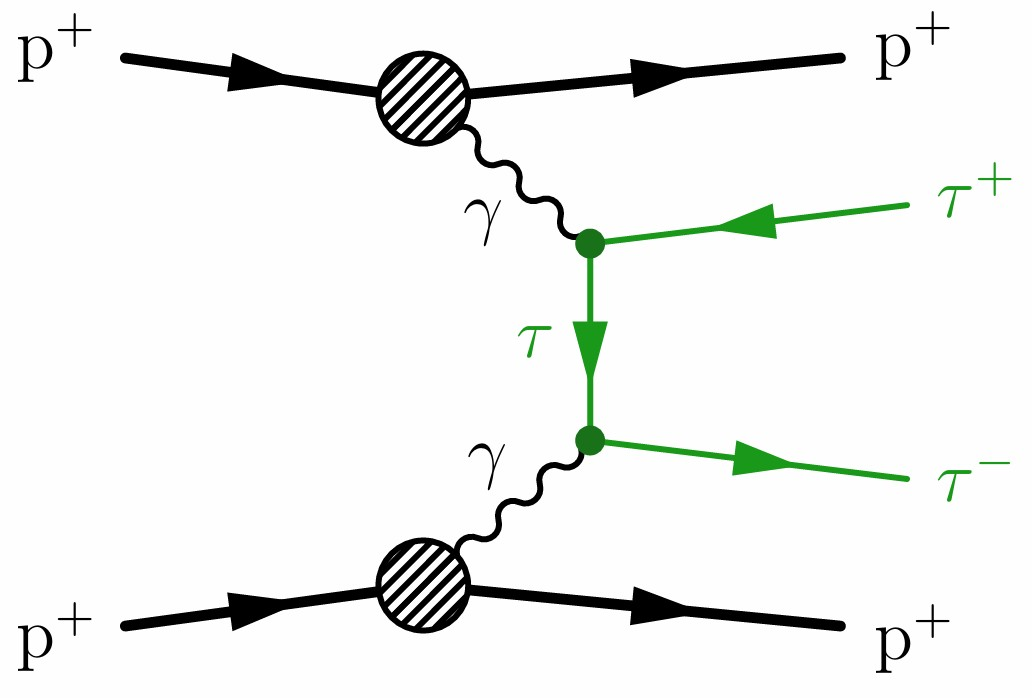
\includegraphics[width=\linewidth]{gg_tautau.jpg}
\caption{\small \justifying Representative topology for photon-induced \(\gamma\gamma \to \tau^+\tau^-\) production in proton-based collisions.}
\end{figure}
\end{column}

\end{columns}
\end{frame}
%=====================================================



\section{Formalism and EFT Interpretation}


%=====================================================
\begin{frame}{General electromagnetic vertex and dipole moments}
\begin{itemize}
 \justifying
  \item The most general on-shell electromagnetic vertex of a charged lepton can be parameterized in terms of form factors:
\end{itemize}
\[
\Gamma^{\mu}(q^2)=\gamma^{\mu}F_1(q^2)+\frac{i\sigma^{\mu\nu}q_{\nu}}{2m_{\tau}}F_2(q^2)+\sigma^{\mu\nu}q_{\nu}\gamma_5\,F_3(q^2).
\]
\begin{itemize}
  \justifying
    \item At zero momentum transfer, the static electromagnetic moments are identified through
\end{itemize}
\[
\textcolor{TauBlue}{F_2(0)=\atau},
\qquad
\textcolor{TauGreen}{F_3(0)=-\frac{2m_{\tau}}{e}\,\dtau}.
\]
\begin{block}{Interpretation}
\small
 \justifying
\textcolor{TauBlue}{\atau} measures the anomalous magnetic dipole moment, while \textcolor{TauGreen}{\dtau} measures the electric dipole moment and is CP-odd.
\end{block}
\end{frame}
%=====================================================




%=====================================================
\begin{frame}{Low-energy dipole interaction for the $\gamma\tau\tau$ vertex}
\begin{itemize}
 \justifying
    \item At the effective-interaction level, the anomalous electromagnetic moments are captured by a dipole-type term in the Lagrangian:
\end{itemize}
\[
\mathcal{L}_{\tau\tau\gamma}=\frac{1}{2}\,\bar\tau\sigma^{\mu\nu}
\left(
\textcolor{TauBlue}{\atau}\,\frac{e}{2m_{\tau}}
- i\,\textcolor{TauGreen}{\dtau}\,\gamma_5
\right)\tau\,F_{\mu\nu}.
\]
\begin{itemize}
 \justifying
    \item The magnetic contribution is CP-even and the electric-dipole contribution is CP-odd.
    \item In a collider process such as \(\gamma\gamma\to\tau^+\tau^-\), these couplings change both the overall rate and the shape of kinematic distributions.
    \item In practice, the mass spectrum is the cleanest place to see the corresponding BSM distortion.
\end{itemize}
\takehome{
 \justifying The talk focuses on the benchmark \(\datau=0.008\), keeping the emphasis on the magnetic-moment sensitivity.}
\end{frame}
%=====================================================



%=====================================================
\begin{frame}{SMEFT interpretation of anomalous $\tau$ moments}
\begin{columns}[T,onlytextwidth]
%---------------- left column ----------------
\begin{column}{0.77\textwidth}
\begin{itemize}
\justifying
\item In the SMEFT language, the relevant dim-6 operators can be written as
\end{itemize}
\[
\mathcal{L}_{\mathrm{BSM}}=
\bar L_{\tau}\sigma^{\mu\nu}\tau_R H
\left[
\textcolor{TauOrange}{\frac{\ctb}{\Lam^2}} B_{\mu\nu}
+
\textcolor{TauOrange}{\frac{\ctw}{\Lam^2}} W_{\mu\nu}
\right]+\mathrm{h.c.}
\]
\begin{itemize}
\justifying
\item After electroweak symmetry breaking, the physical photon combination appears through a linear combination of the Wilson coefficients.
\item The real part gives the CP-even magnetic deformation and the imaginary part gives the CP-odd electric-dipole deformation.
\end{itemize}
\[
\textcolor{TauBlue}{\ddtau}=\frac{\sqrt2\,v}{\Lam^2}\,\mathrm{Im}\!\left[\cos\theta_W\,\ctb-\sin\theta_W\,\ctw\right],
\]
\[
\textcolor{TauBlue}{\datau}=\frac{2m_{\tau}}{e}\,\frac{\sqrt2\,v}{\Lam^2}\,\mathrm{Re}\!\left[\cos\theta_W\,\ctb-\sin\theta_W\,\ctw\right].
\]
\end{column}
%---------------- right column ----------------
\begin{column}{0.20\textwidth}
\vspace*{3.0cm}
\centering
\hspace*{0.4cm}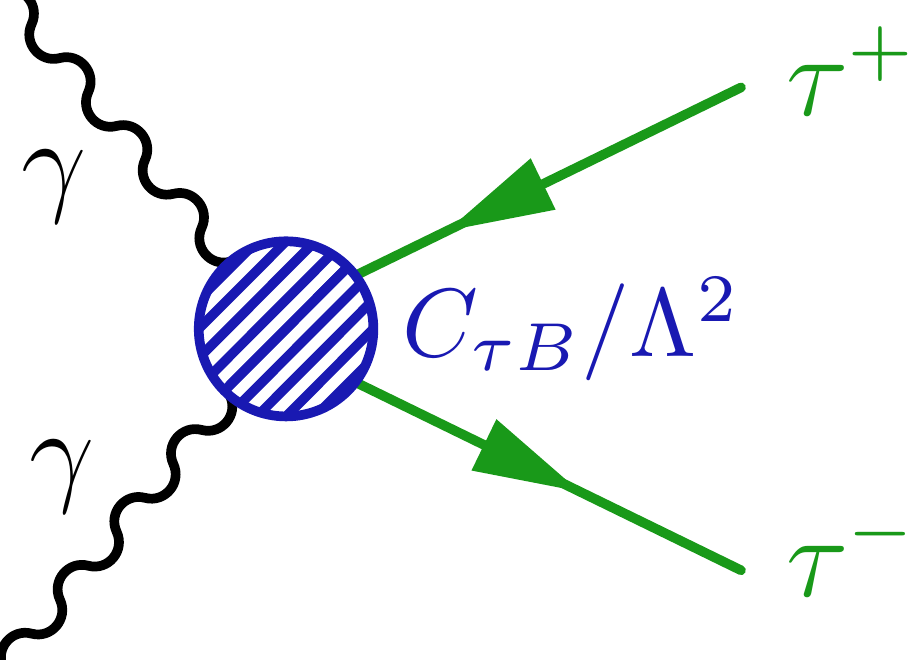
\includegraphics[width=\linewidth]{Ctb.png}
\vspace{0.3em}
{\scriptsize
Dipole-type SMEFT insertion associated with \(\ctb/\Lam^2\).
}
\end{column}
\end{columns}
\end{frame}
%=====================================================



%=====================================================
\begin{frame}{Benchmark implementation used in this study}
\begin{columns}[T]
\begin{column}{0.65\textwidth}
\begin{itemize}
\justifying
\item Event generation is performed with the {\color{red}\texttt{SMEFTsim\_top\_alphaScheme\_UFO}} model.
\item The present local benchmark corresponds to a nonzero CP-even dipole deformation associated with the tau sector and interpreted as \(\datau=0.008\).
\item In the local banners, the BSM benchmark is realized using a nonzero tau dipole Wilson-coefficient entry and \(\Lam= {\color{red}2}~\mathrm{TeV}\) for the EFT normalization.
\item The study is designed as a {\color{blue}truth-level comparison} between the SM and a single illustrative BSM benchmark, not yet as a detector-level limit extraction.
\end{itemize}
\end{column}
\begin{column}{0.36\textwidth}
\begin{block}{Color legend}
\small
\begin{itemize}
\justifying
\item \textcolor{TauBlue}{\(\atau,\ \datau\)}: magnetic moment sector
\item \textcolor{TauGreen}{\(\dtau,\ \ddtau\)}: electric dipole sector
\item \textcolor{TauOrange}{\(\ctb,\ctw,\Lam\)}: EFT parameters
\end{itemize}
\end{block}
\end{column}
\end{columns}
\end{frame}
%=====================================================



% Optional style (put once in the preamble if not already defined)
\tikzset{
	eftcircle/.style={
		circle,
		draw=TauBlue,
		line width=1.3pt,
		fill=white,
		pattern=north east lines,
		pattern color=TauBlue,
		minimum size=2mm,
		inner sep=0pt
	}
}

%=====================================================
\begin{frame}{Amplitude structure and representative diagrams}
	
\begin{columns}[T,onlytextwidth]
%------------------------------------------------
\begin{column}{0.28\textwidth}
\centering
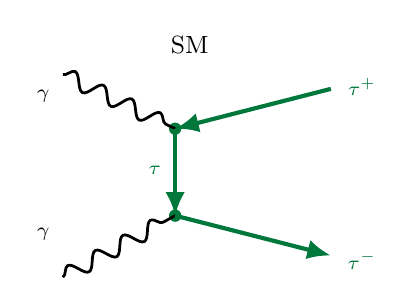
\begin{tikzpicture}[scale=0.92]
\node at (0.2,3.15) {\small SM};
				
				% vertices
				\fill[TauGreen] (0,2.0) circle (0.085);
				\fill[TauGreen] (0,0.8) circle (0.085);
				
				% photons
				\draw[photon] (-1.55,2.75) -- (0,2.0);
				\draw[photon] (-1.55,-0.05) -- (0,0.8);
				
				% fermion lines
				\draw[TauGreen,line width=1.5pt,-{Latex[length=3mm,width=2.5mm]}] (0,2.0) -- (0,0.8);
				\draw[TauGreen,line width=1.5pt,{Latex[length=3mm,width=2.5mm]}-] (0,2.0) -- (2.15,2.55);
				\draw[TauGreen,line width=1.5pt,-{Latex[length=3mm,width=2.5mm]}] (0,0.8) -- (2.15,0.25);
				
				% labels
				\node at (-1.82,2.45) {\scriptsize $\gamma$};
				\node at (-1.82,0.55) {\scriptsize $\gamma$};
				\node[TauGreen] at (-0.28,1.42) {\scriptsize $\tau$};
				\node[TauGreen] at (2.58,2.58) {\scriptsize $\tau^{+}$};
				\node[TauGreen] at (2.58,0.18) {\scriptsize $\tau^{-}$};
\end{tikzpicture}
\end{column}
%------------------------------------------------
\begin{column}{0.28\textwidth}
\centering
\begin{tikzpicture}[scale=0.92]
\node at (0.2,3.15) {\small linear BSM insertion};
				
				% vertices
				\fill[TauGreen] (0,2.0) circle (0.085);
				\fill[TauGreen] (0,0.8) circle (0.085);
				
				% EFT insertion (one circle)
				\node[eftcircle] at (0,2.0) {};
				
				% photons
				\draw[photon] (-1.55,2.75) -- (0,2.0);
				\draw[photon] (-1.55,-0.05) -- (0,0.8);
				
				% fermion lines
				\draw[TauGreen,line width=1.5pt,-{Latex[length=3mm,width=2.5mm]}] (0,2.0) -- (0,0.8);
				\draw[TauGreen,line width=1.5pt,{Latex[length=3mm,width=2.5mm]}-] (0,2.0) -- (2.15,2.55);
				\draw[TauGreen,line width=1.5pt,-{Latex[length=3mm,width=2.5mm]}] (0,0.8) -- (2.15,0.25);
				
				% labels
				\node at (-1.82,2.45) {\scriptsize $\gamma$};
				\node at (-1.82,0.55) {\scriptsize $\gamma$};
				\node[TauGreen] at (-0.28,1.42) {\scriptsize $\tau$};
				\node[TauGreen] at (2.58,2.58) {\scriptsize $\tau^{+}$};
				\node[TauGreen] at (2.58,0.18) {\scriptsize $\tau^{-}$};
\end{tikzpicture}
\end{column}
%------------------------------------------------
\begin{column}{0.28\textwidth}
\centering
\begin{tikzpicture}[scale=0.92]
				\node at (0.2,3.15) {\small quadratic BSM term};
				
				% vertices
				\fill[TauGreen] (0,2.0) circle (0.085);
				\fill[TauGreen] (0,0.8) circle (0.085);
				
				% EFT insertions (two circles)
				\node[eftcircle] at (0,2.0) {};
				\node[eftcircle] at (0,0.8) {};
				
				% photons
				\draw[photon] (-1.55,2.75) -- (0,2.0);
				\draw[photon] (-1.55,-0.05) -- (0,0.8);
				
				% fermion lines
				\draw[TauGreen,line width=1.5pt,-{Latex[length=3mm,width=2.5mm]}] (0,2.0) -- (0,0.8);
				\draw[TauGreen,line width=1.5pt,{Latex[length=3mm,width=2.5mm]}-] (0,2.0) -- (2.15,2.55);
				\draw[TauGreen,line width=1.5pt,-{Latex[length=3mm,width=2.5mm]}] (0,0.8) -- (2.15,0.25);
				
				% labels
				\node at (-1.82,2.45) {\scriptsize $\gamma$};
				\node at (-1.82,0.55) {\scriptsize $\gamma$};
				\node[TauGreen] at (-0.28,1.42) {\scriptsize $\tau$};
				\node[TauGreen] at (2.58,2.58) {\scriptsize $\tau^{+}$};
				\node[TauGreen] at (2.58,0.18) {\scriptsize $\tau^{-}$};
\end{tikzpicture}
\end{column}
%------------------------------------------------
\end{columns}
\vspace{1.0ex}
\begin{block}{Interpretation of the generated samples}
\justifying
\small
The SM sample is generated with \texttt{NP=0}. The benchmark BSM sample is generated with \texttt{NP<=2}, so the prediction includes the Standard Model contribution together with the interference term and the quadratic EFT contribution in the MadGraph operator-order convention used in this study.
\end{block}
	
\end{frame}
%=====================================================



\section{Collider Setups and Event Generation}


%=====================================================
\begin{frame}{Future lepton-hadron collider program considered here}
\begin{columns}[T]
\begin{column}{0.49\textwidth}
\begin{block}{LHeC}
\begin{itemize}
 \justifying
    \item proton beam: \(E_p=7~\mathrm{TeV}\)
    \item electron beam: \(E_e=50~\mathrm{GeV}\)
    \item center-of-mass energy: \(\sqrt{s}\approx 1.2~\mathrm{TeV}\)
\end{itemize}
\end{block}
\end{column}
\begin{column}{0.49\textwidth}
\begin{block}{LH$\mu$C}
\begin{itemize}
 \justifying
    \item proton beam: \(E_p=7~\mathrm{TeV}\)
    \item antimuon / \(\mu^+\) beam in the local MadGraph setup: \(E_{\mu}=500~\mathrm{GeV}\)
    \item center-of-mass energy: \(\sqrt{s}\approx 3.7~\mathrm{TeV}\)
\end{itemize}
\end{block}
\end{column}
\end{columns}
\begin{itemize}
\justifying
\item The present study keeps the comparison symmetric: the same process, the same EFT benchmark, and the same LHE-level analysis logic are used for both colliders.
\item This makes the difference in the observed BSM distortion directly interpretable as a collider-environment effect within the current setup.
\end{itemize}
\end{frame}
%=====================================================




%=====================================================
\begin{frame}[fragile]{MadGraph process definition and sample types}
\begin{columns}[T]
\begin{column}{0.52\textwidth}
\begin{block}{SM generation}
\scriptsize\ttfamily
import model SMEFTsim\_top\_alphaScheme\_UFO\\
\vspace{0.4ex}
generate a a > ta+ ta- / h h1 NP=0 SMHLOOP=0
\end{block}
\begin{block}{BSM benchmark generation}
\scriptsize\ttfamily
import model SMEFTsim\_top\_alphaScheme\_UFO\\
\vspace{0.4ex}
generate a a > ta+ ta- / h h1 NP<=2 SMHLOOP=0
\end{block}
\end{column}
\begin{column}{0.50\textwidth}
\begin{itemize}
\justifying
\item The hard process is identical in the two colliders; only the beam configuration changes.
\item \texttt{NP=0} isolates the SM contribution.
\item \texttt{NP<=2} includes the benchmark BSM effects together with the SM piece in the operator-order counting used in the model.
\item This is especially important in the hard tail, where quadratic contributions can visibly enhance the spectrum.
\end{itemize}
\end{column}
\end{columns}
\end{frame}
%=====================================================




%=====================================================
\begin{frame}[fragile]{Beam configuration and run-card logic}
\begin{columns}[T]
\begin{column}{0.49\textwidth}
\begin{block}{LHeC banner essentials}
\scriptsize\ttfamily
lpp1 = 2\\
lpp2 = 3\\
ebeam1 = 7000.0\\
ebeam2 = 50.0\\
pdlabel1 = iww\\
pdlabel2 = iww
\end{block}
\end{column}
\begin{column}{0.49\textwidth}
\begin{block}{LHmuC banner essentials}
\scriptsize\ttfamily
lpp1 = 2\\
lpp2 = -4\\
ebeam1 = 7000.0\\
ebeam2 = 500.0\\
pdlabel1 = iww\\
pdlabel2 = iww
\end{block}
\end{column}
\end{columns}
\vspace{1cm}
\begin{itemize}
\justifying
\item The current local setup uses an equivalent-photon description of the beams through the \texttt{iww} choice.
\item This is therefore a generator-level truth study using an effective photon-emission picture, not a full detector simulation.
\end{itemize}
\end{frame}
%=====================================================




%=====================================================
\begin{frame}[fragile]{Generation cuts, benchmark choice, and statistics}
\begin{columns}[T]
\begin{column}{0.52\textwidth}
\begin{block}{Run-card highlights}
\scriptsize\ttfamily
mmll = 10.0\\
ptl = -1.0\\
etal = -1.0\\
drll = -1.0
\end{block}
\begin{itemize}
 \justifying
    \item The generation is largely inclusive, with a minimal invariant-mass cut \(m_{\ell\ell}>10~\mathrm{GeV}\).
    \item No strong truth-level acceptance cuts are imposed on lepton transverse momentum, rapidity, or separation at generation.
\end{itemize}
\end{column}
\begin{column}{0.44\textwidth}
\begin{block}{Sample statistics}
\begin{itemize}
 \justifying
    \item 5 independent runs per sample
    \item 1M unweighted events per run
    \item 5M events per collider and per hypothesis
    \item LHE header cross sections combined with event-count weighting
\end{itemize}
\end{block}
\begin{exampleblock}{Benchmark}
\small Present comparison: \(\datau=0.008\) at truth level.
\end{exampleblock}
\end{column}
\end{columns}
\end{frame}
%=====================================================



%=====================================================
\begin{frame}{Benchmark cross sections and Monte Carlo luminosities}
\centering
\begin{tabular}{>{\raggedright\arraybackslash}p{0.28\textwidth}ccc}
\toprule
Sample & $\sigma_{\mathrm{SM}}$ [pb] & $\sigma_{\mathrm{BSM}}$ [pb] & $N_{\mathrm{events}}$ \\
\midrule
LHeC{\color{magenta}@}1.2 TeV & 50.695 & 51.923 & $5\times10^6$ \\
LH$\mu$C{\color{magenta}@}3.7 TeV & 55.094 & 56.461 & $5\times10^6$ \\
\bottomrule
\end{tabular}

\vspace{1em}
\begin{itemize}
\justifying
\item The effective luminosities inferred from the Monte Carlo sample sizes are approximately \(97.5~\mathrm{fb}^{-1}\) for the LHeC benchmark and \(89.7~\mathrm{fb}^{-1}\) for the LH$\mu$C benchmark.
\item These values are {\color{red}{Monte Carlo effective luminosities}} used for the plot normalization logic; they are not the final projected machine luminosities for a full experimental analysis.
\end{itemize}
\end{frame}
%=====================================================


\section{Analysis Strategy}


%=====================================================
\begin{frame}{Truth-level analysis workflow implemented in the local code}
\begin{enumerate}
 \justifying
    \item Read all \texttt{run\_*} LHE or LHE.GZ files under the corresponding \texttt{Events/} directory.
    \item Parse final-state \(\tau^+\) and \(\tau^-\) four-momenta from each event.
    \item Construct the pair observables \(\Mtt\) and \(\Ytt\).
    \item Convert binned event counts into weighted differential spectra using the LHE cross section.
    \item Build the physical BSM/SM ratio from \((d\sigma/dM)_{\mathrm{BSM}}\) and \((d\sigma/dM)_{\mathrm{SM}}\).
    \item Also build legacy count-ratio plots to keep continuity with earlier visualizations.
    \item Fit the ratio using a linear ansatz \(y(M)=aM+b\) to summarize tail hardening.
\end{enumerate}
\begin{block}{Interpretation of the fit slope}
 \justifying
\small A positive slope indicates that the BSM enhancement grows toward larger \(\Mtt\), i.e. the anomalous coupling hardens the invariant-mass tail.
\end{block}
\end{frame}
%=====================================================



%=====================================================
\begin{frame}{Observables used in the comparison}
\begin{columns}[T]
\begin{column}{0.50\textwidth}
\begin{block}{Primary observables}
\[
\frac{d\sigma}{d\Mtt} (\frac{pb}{GeV}),
\qquad
\frac{d\sigma}{d\Ytt} (\frac{pb}{GeV}),
\]
\begin{itemize}
 \justifying
    \item The invariant-mass spectrum is expected to be the most sensitive observable.
    \item The rapidity distribution is useful as a complementary shape diagnostic.
\end{itemize}
\end{block}
\end{column}
\begin{column}{0.50\textwidth}
\begin{block}{Ratio observables}
\[
\frac{\left(d\sigma/dM\right)_{\mathrm{BSM}}}{\left(d\sigma/dM\right)_{\mathrm{SM}}}
\]
\begin{itemize}
 \justifying
    \item \textbf{Physical weighted ratio}: directly compares the differential spectra.
    \item \textbf{Legacy ratio plots}: retain continuity with the earlier plotting style and support compact linear-fit summaries.
\end{itemize}
\end{block}
\end{column}
\end{columns}
\takehome{
 \justifying
The entire comparison is designed to quantify how strongly the benchmark \(\datau=0.008\) distorts the high-mass shape relative to the Standard Model.}
\end{frame}
%=====================================================


\section{Sensitivity Estimation: LHeC vs LH$\mu$C}


%=====================================================
\begin{frame}{Invariant-mass spectrum: LHeC vs LH$\mu$C}
\begin{figure}
\centering
\begin{minipage}{0.45\textwidth}
\centering
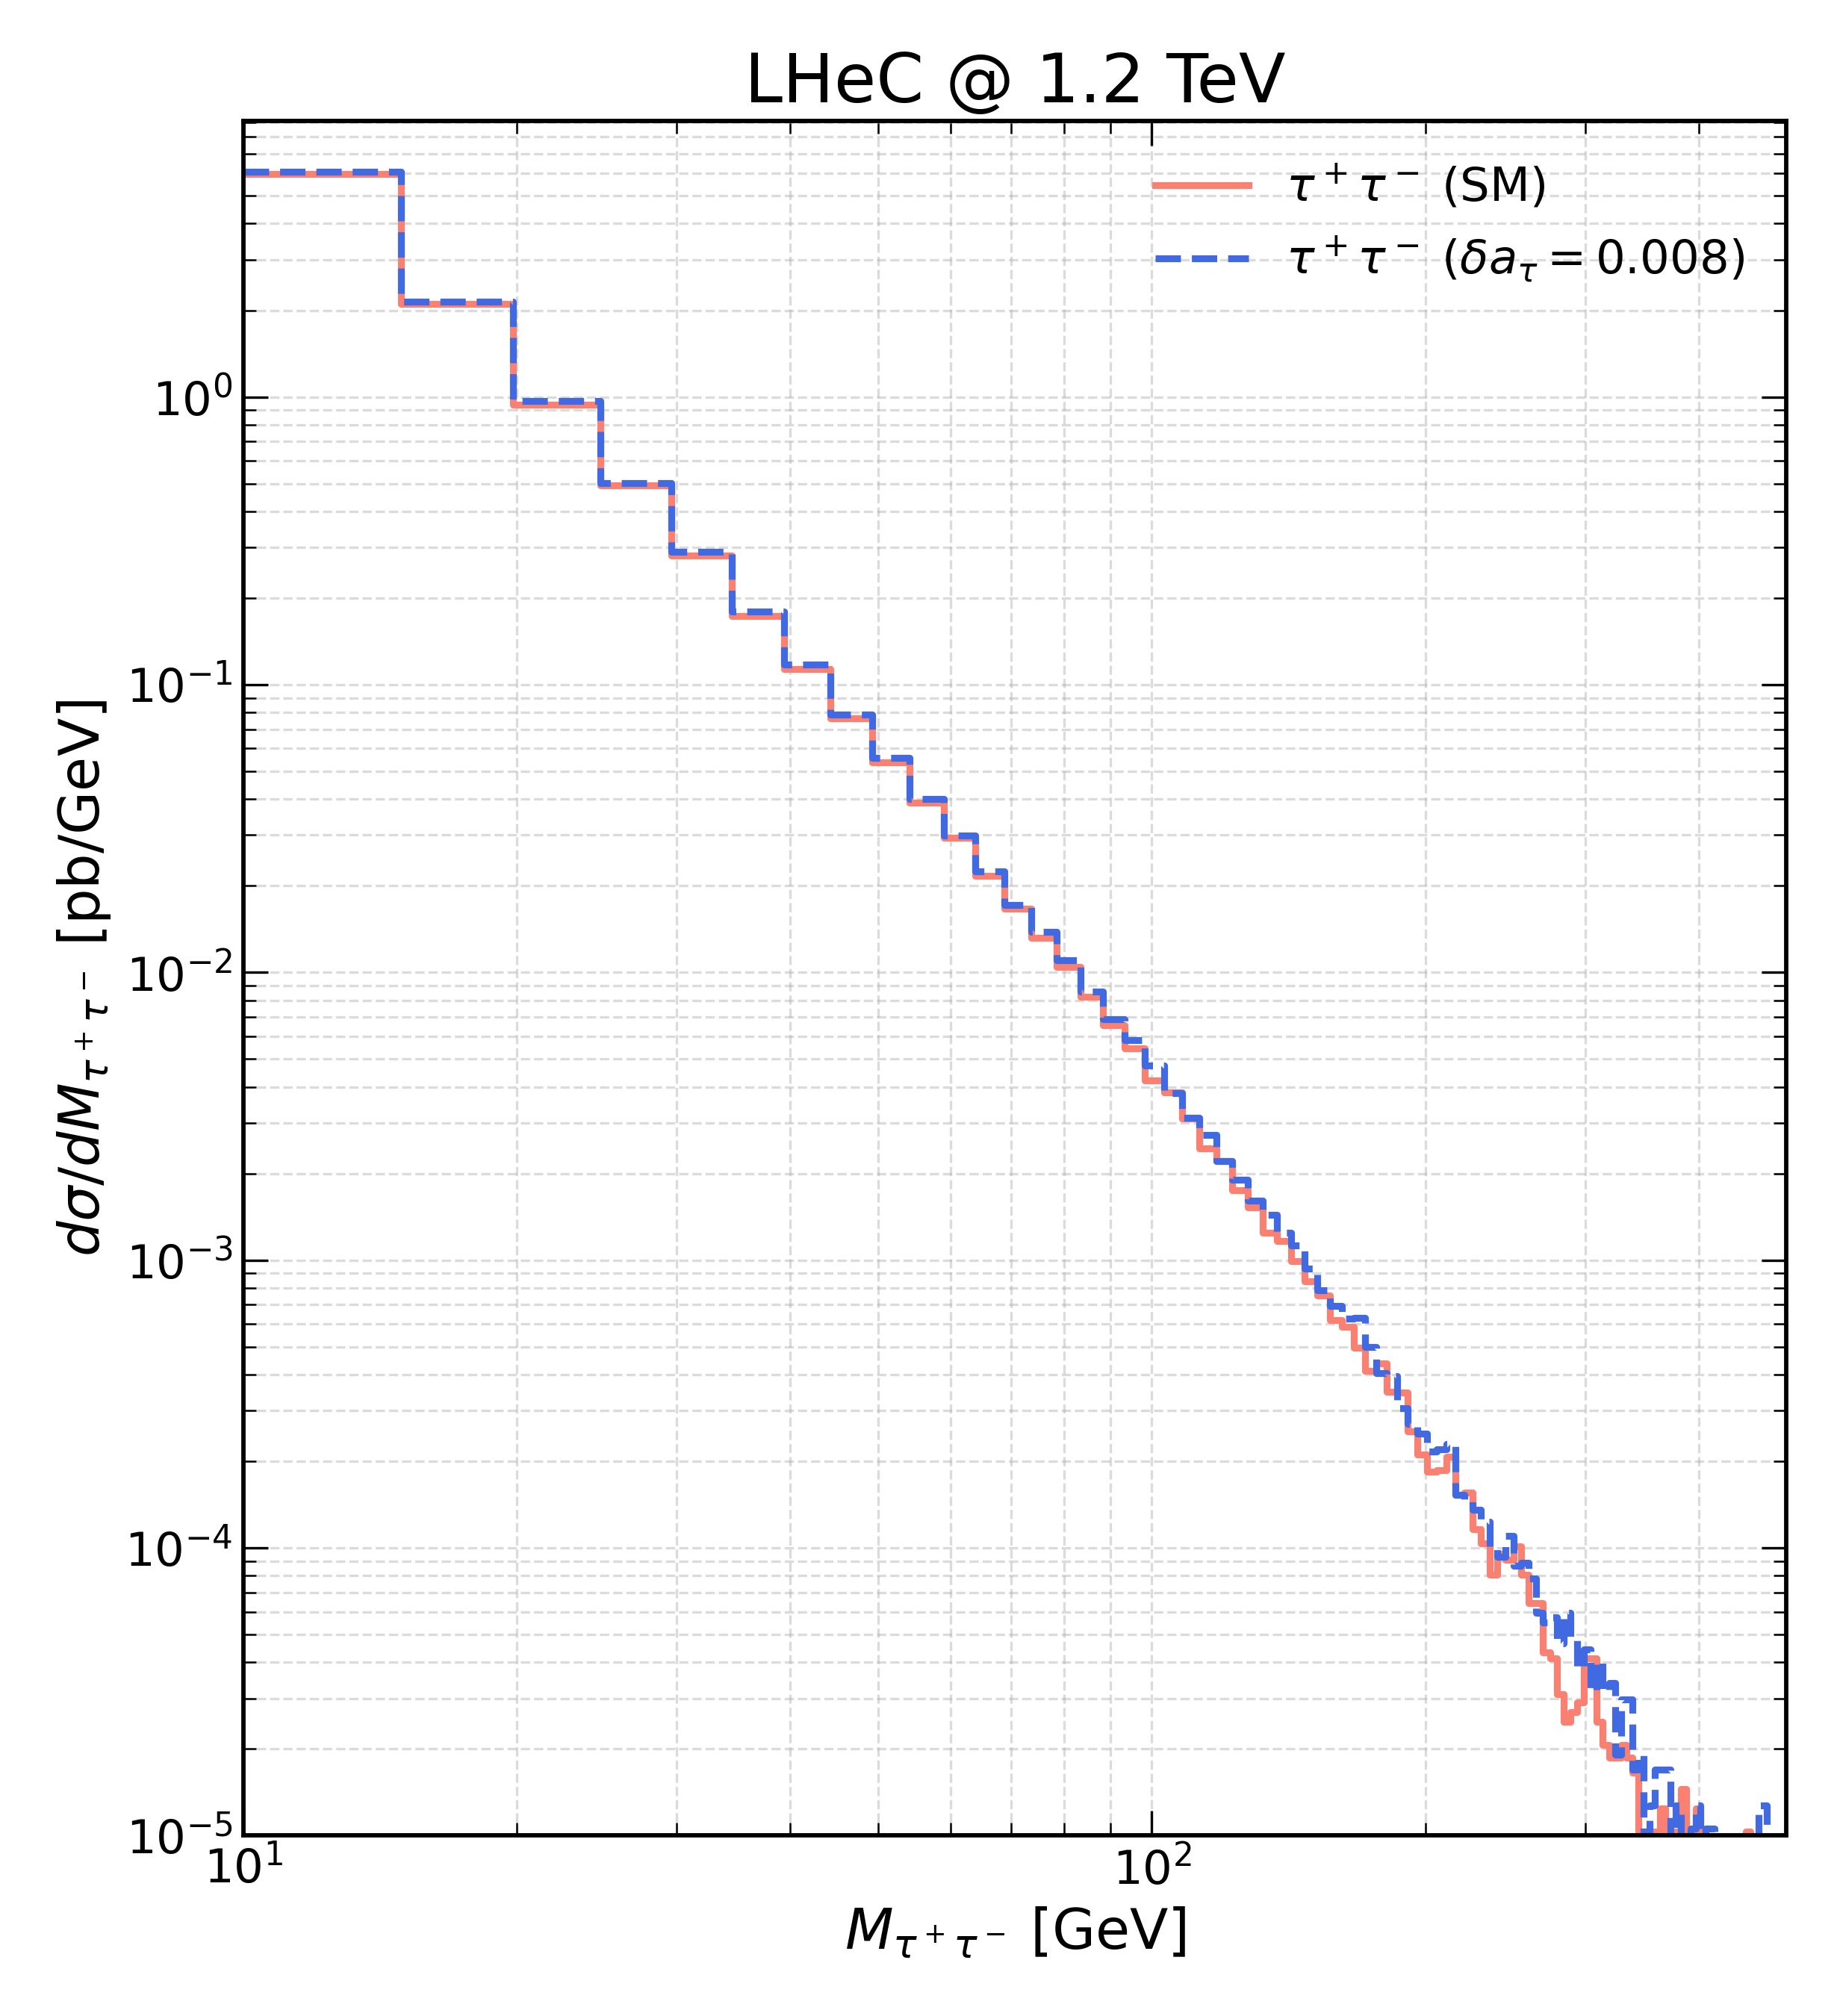
\includegraphics[width=\linewidth]{Invariant_mass_tau_pair_SM_vs_BSM_delta_aTau_LHeC.png}
\end{minipage}
\hfill
\begin{minipage}{0.45\textwidth}
\centering
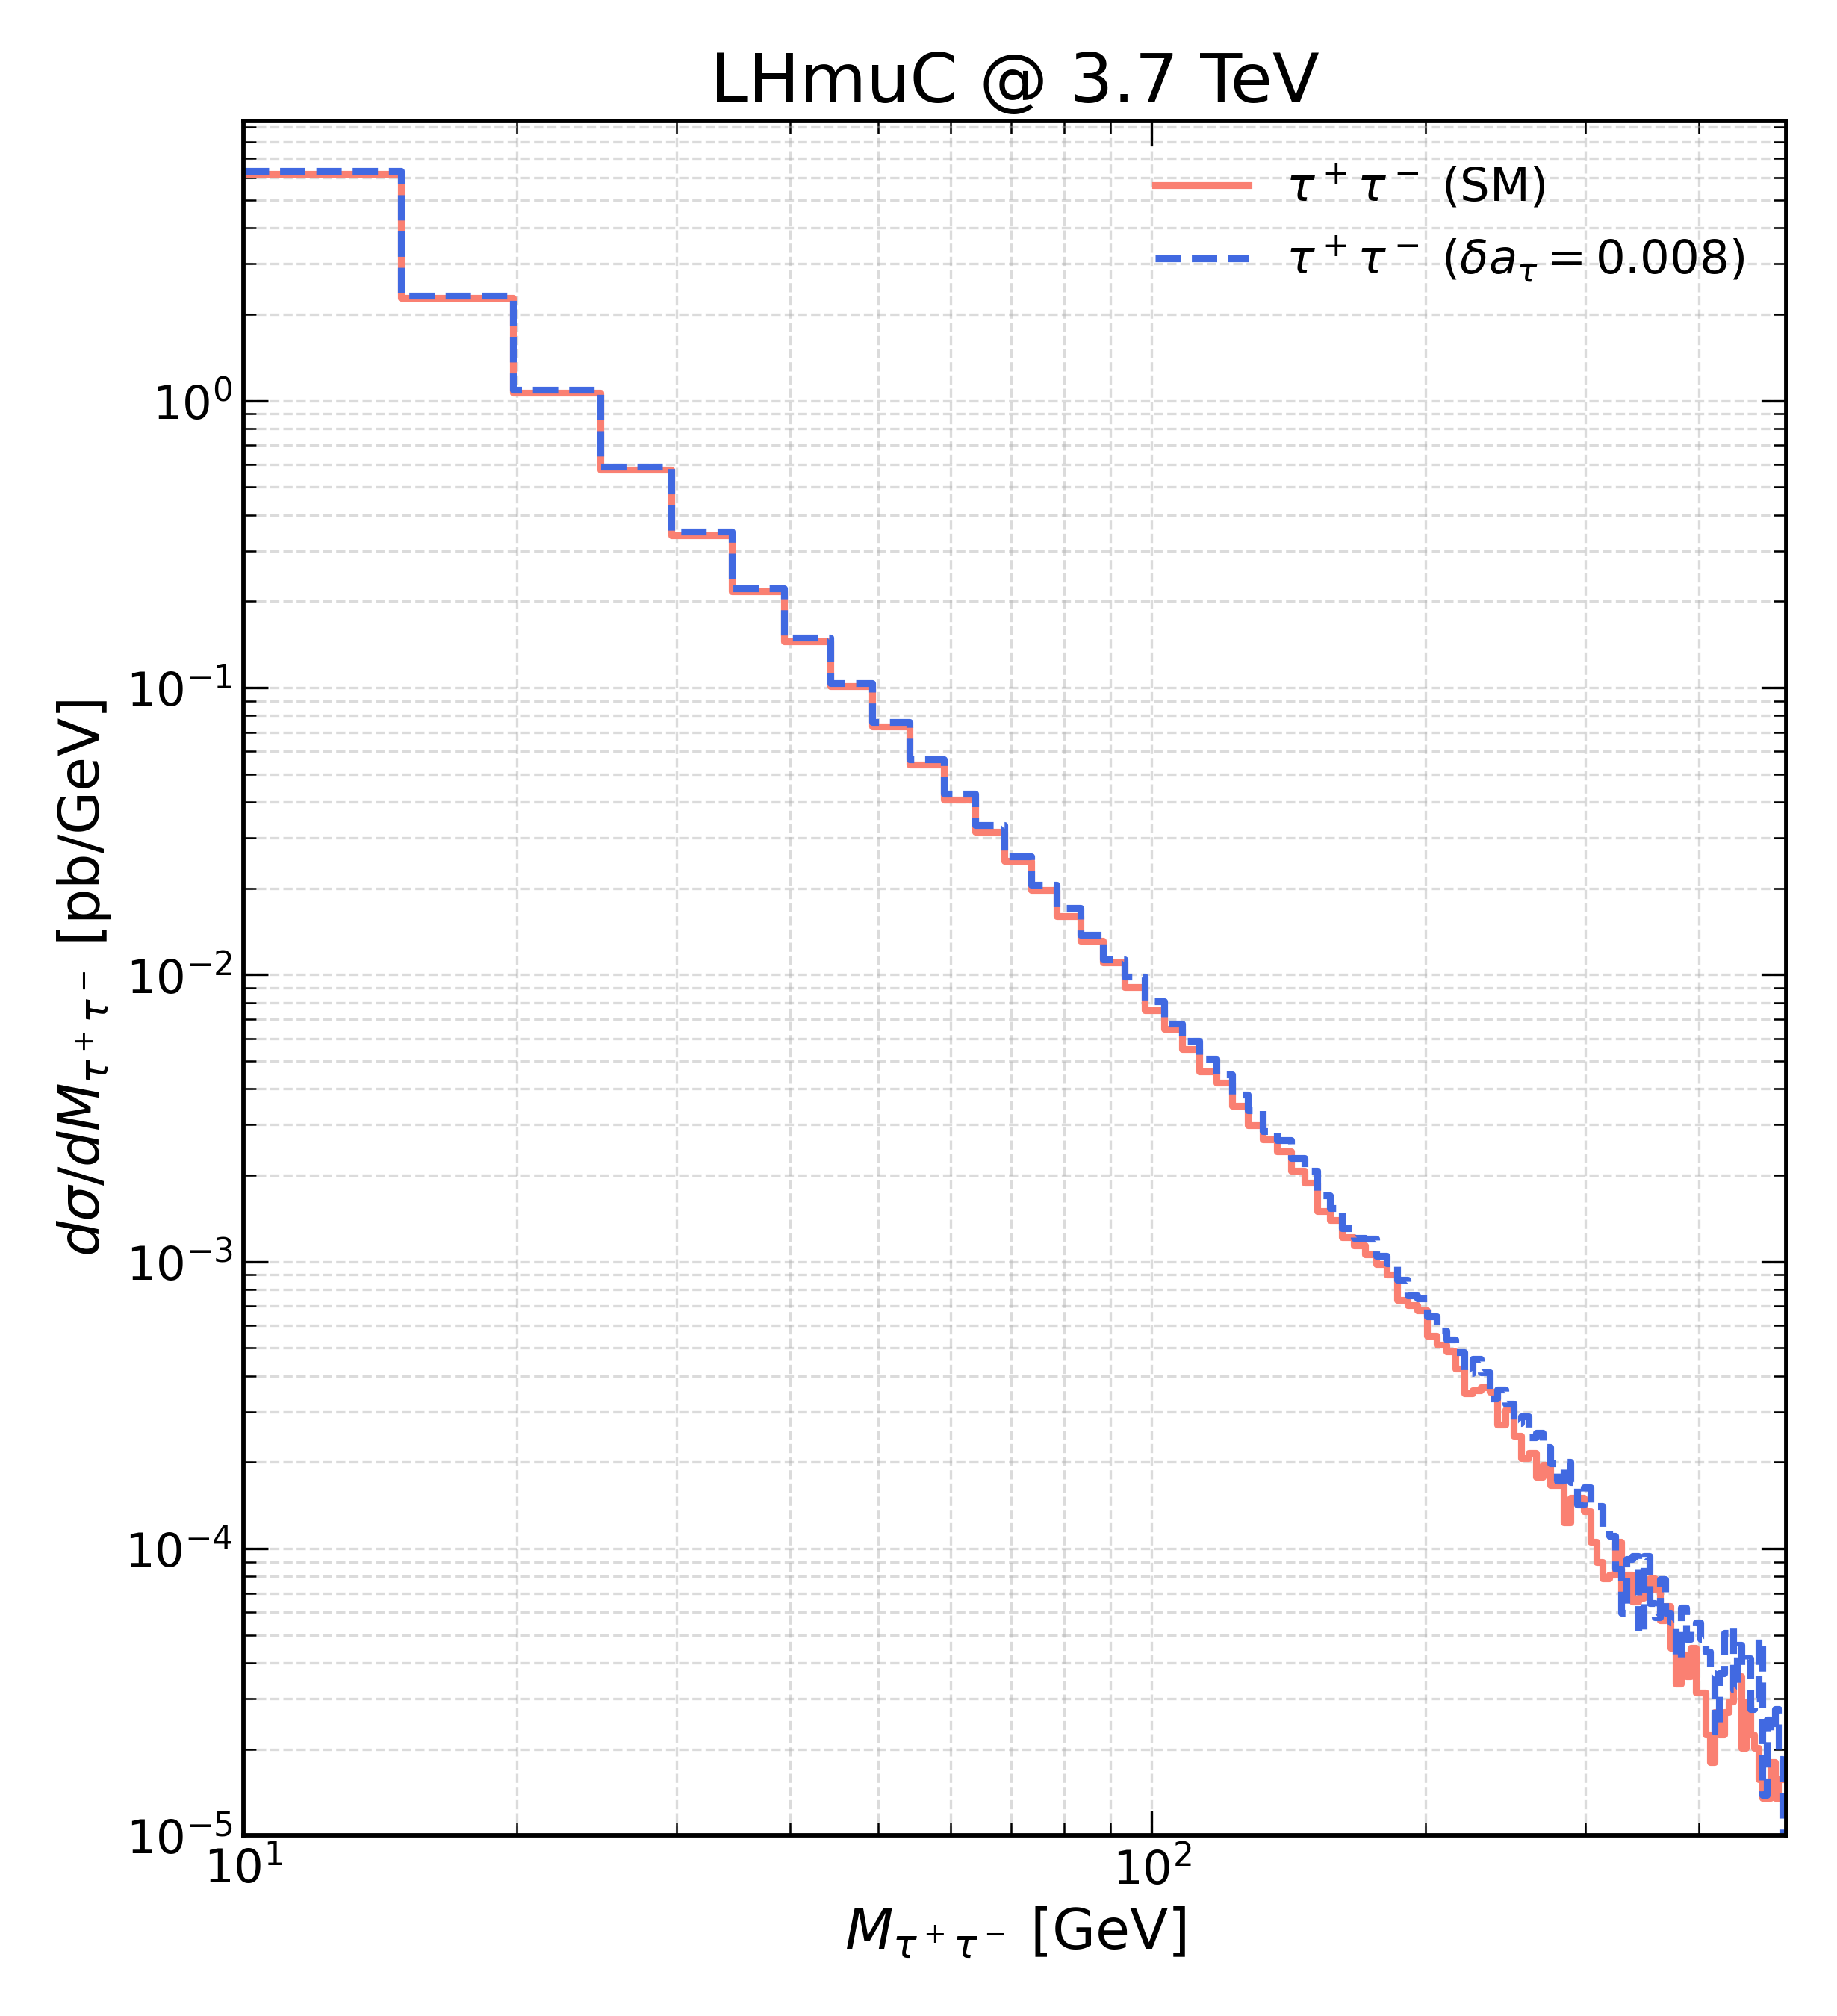
\includegraphics[width=\linewidth]{Invariant_mass_tau_pair_SM_vs_BSM_delta_aTau_LHmuC.png}
\end{minipage}
\caption{\small
\justifying
Comparison of the invariant-mass distributions for photon-induced \(\gamma\gamma \to \tau^+\tau^-\) production at the LHeC and LH$\mu$C for the SM and the benchmark anomalous coupling \(\datau=0.008\). In both cases, the BSM contribution hardens the \(\Mtt\) spectrum relative to the SM expectation.
}
\end{figure}
\end{frame}
%=====================================================

%=====================================================
\begin{frame}{Findings from the invariant-mass comparison}
\begin{itemize}
\justifying
\item In both collider configurations, the benchmark value \(\datau=0.008\) produces a harder \(\Mtt\) spectrum than the Standard Model prediction.
\item The separation between the SM and BSM curves becomes increasingly visible toward larger invariant mass, showing that the anomalous dipole contribution mainly affects the hard tail.
\item This trend is physically expected, since dipole-type interactions become more important at higher momentum transfer.
\item The effect is more pronounced for the LH$\mu$C, where the BSM enhancement in the high-\(\Mtt\) region is visibly stronger than in the LHeC case.
\item Therefore, already at the level of the invariant-mass spectrum, the LH$\mu$C appears more sensitive to anomalous \(\tau\)-dipole effects in the present truth-level benchmark setup.
\end{itemize}
	
\takehome{
\justifying
The invariant-mass tail is the most discriminating observable in this study, and its stronger deformation at the {\color{red} LH$\mu$C already suggests a better sensitivity to \atau\ than at the LHeC}.
}
\end{frame}
%=====================================================



%=====================================================
\begin{frame}{Rapidity distribution: LHeC vs LH$\mu$C}
\begin{columns}[T,onlytextwidth]
\begin{column}{0.45\textwidth}
\centering
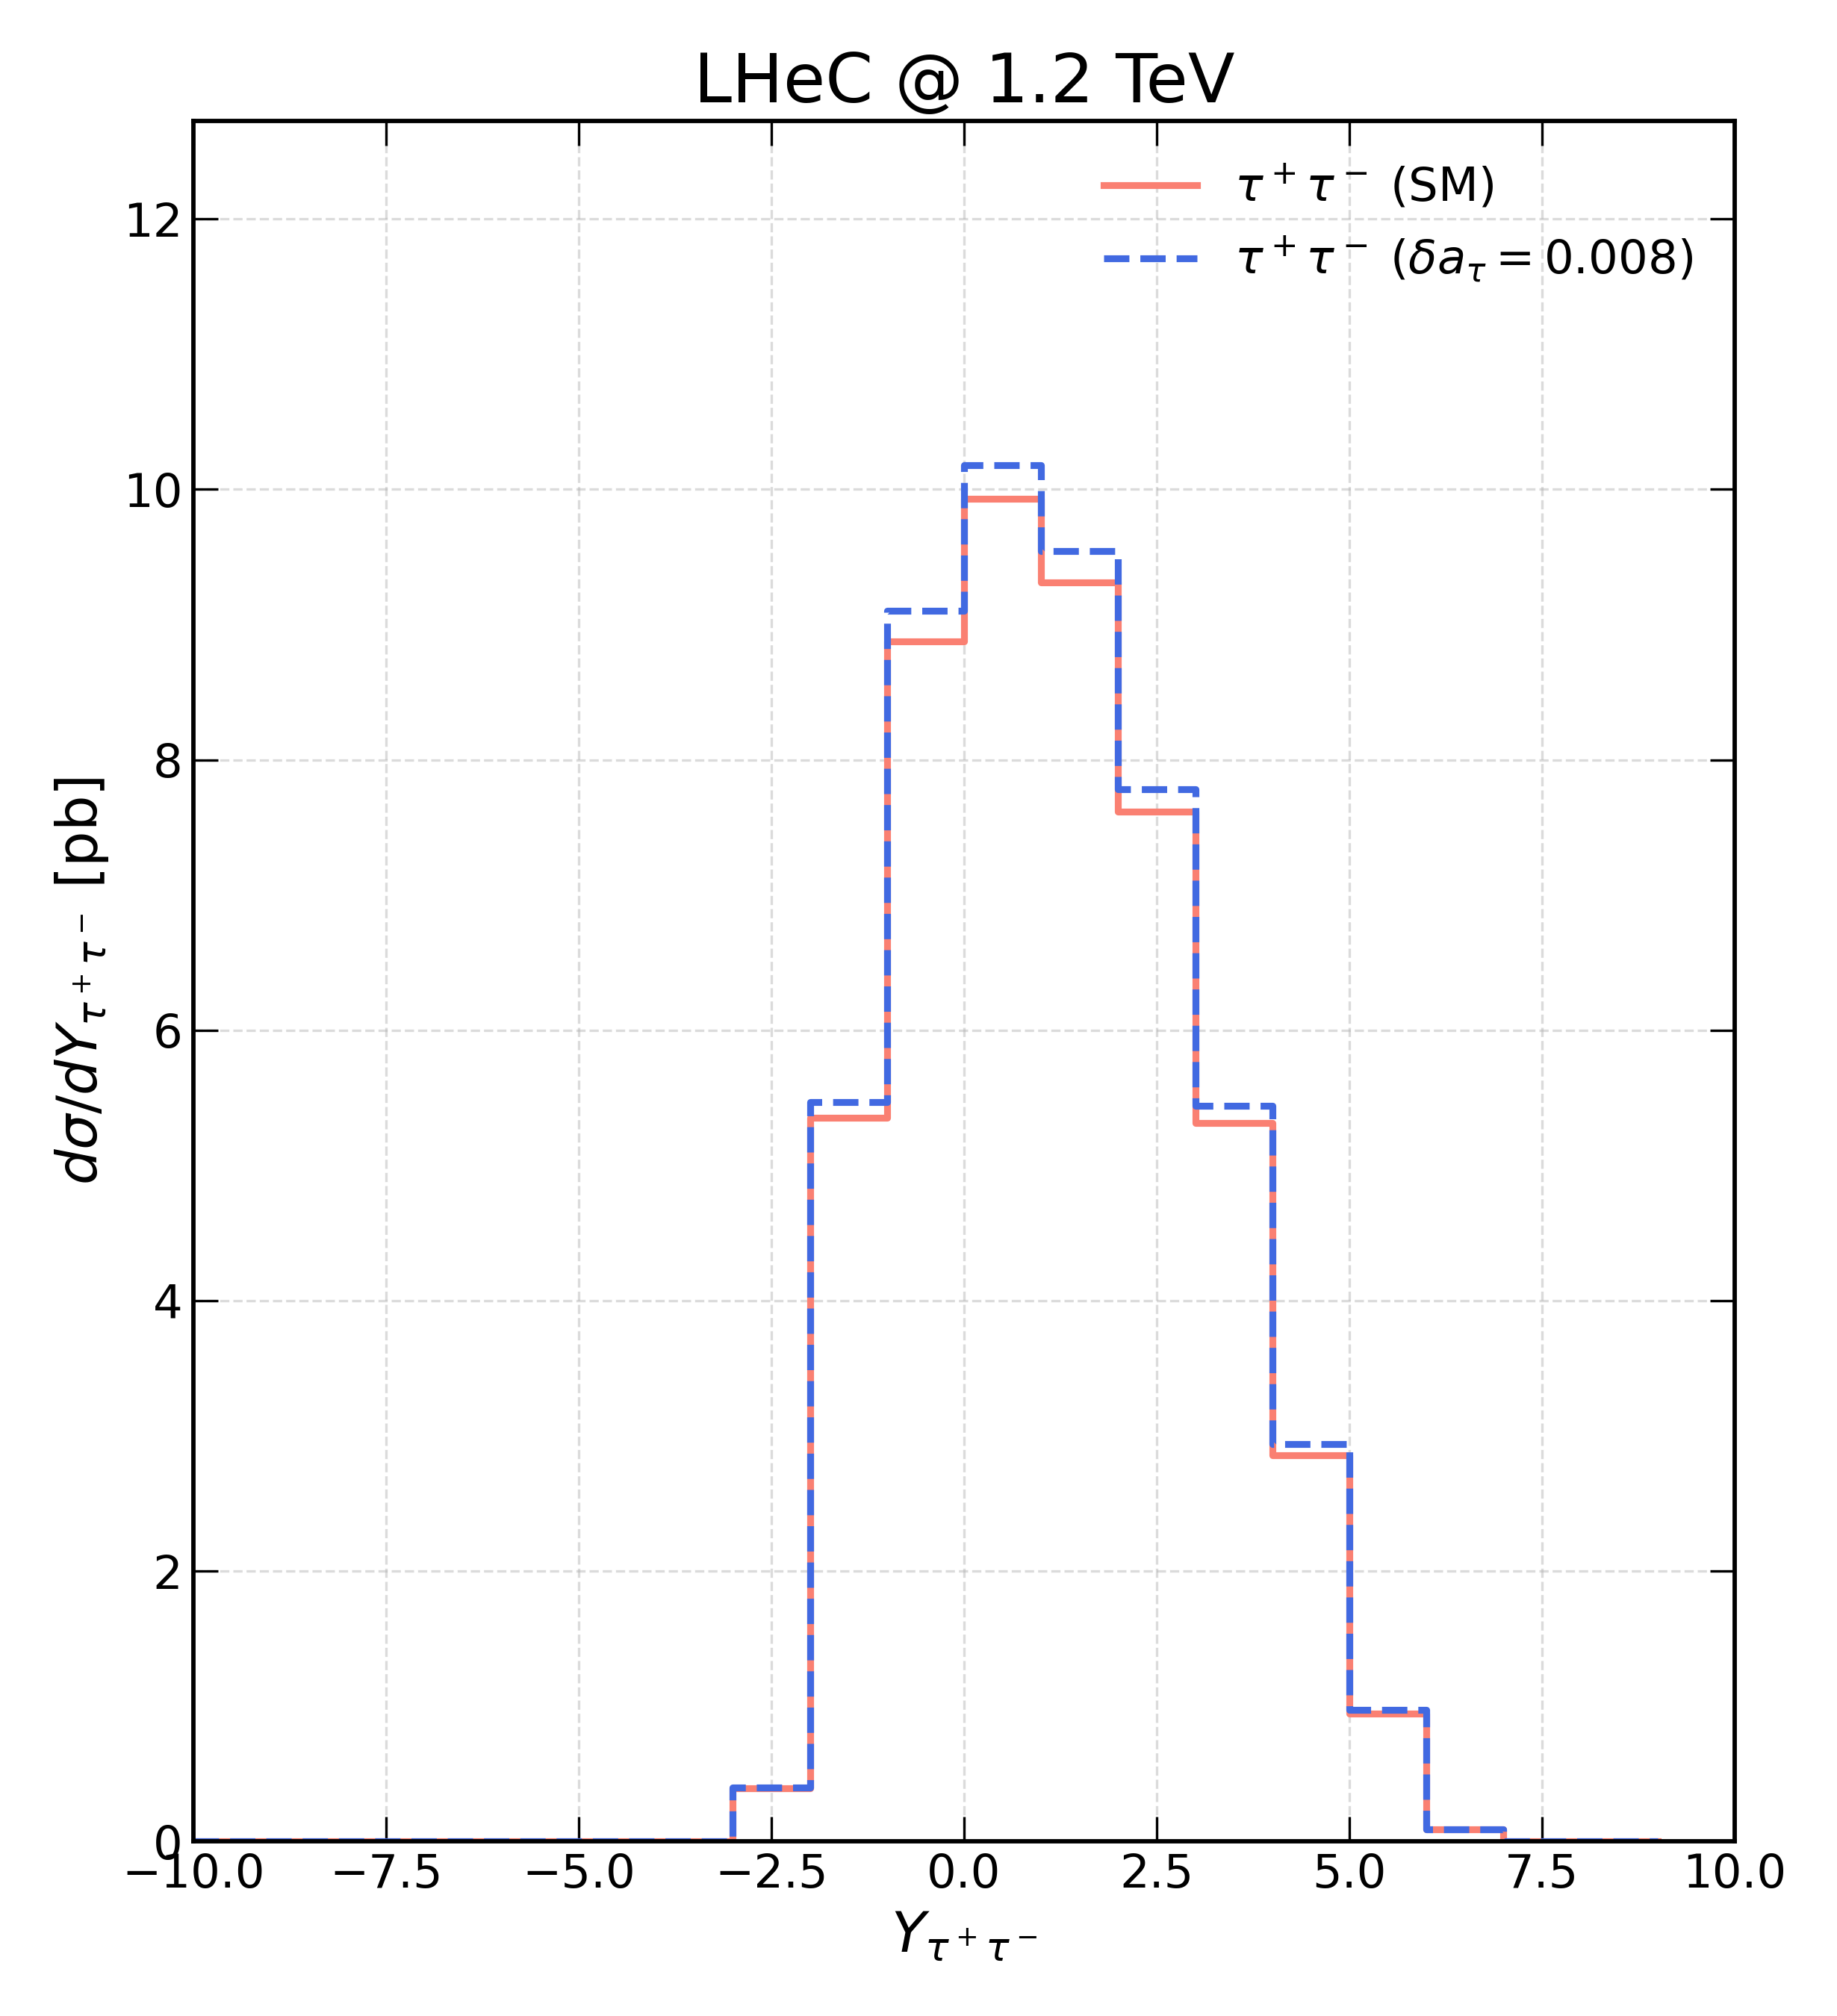
\includegraphics[width=\linewidth]{Rapidity_tau_pair_SM_vs_BSM_delta_aTau_LHeC.png}
\end{column}
\begin{column}{0.45\textwidth}
\centering
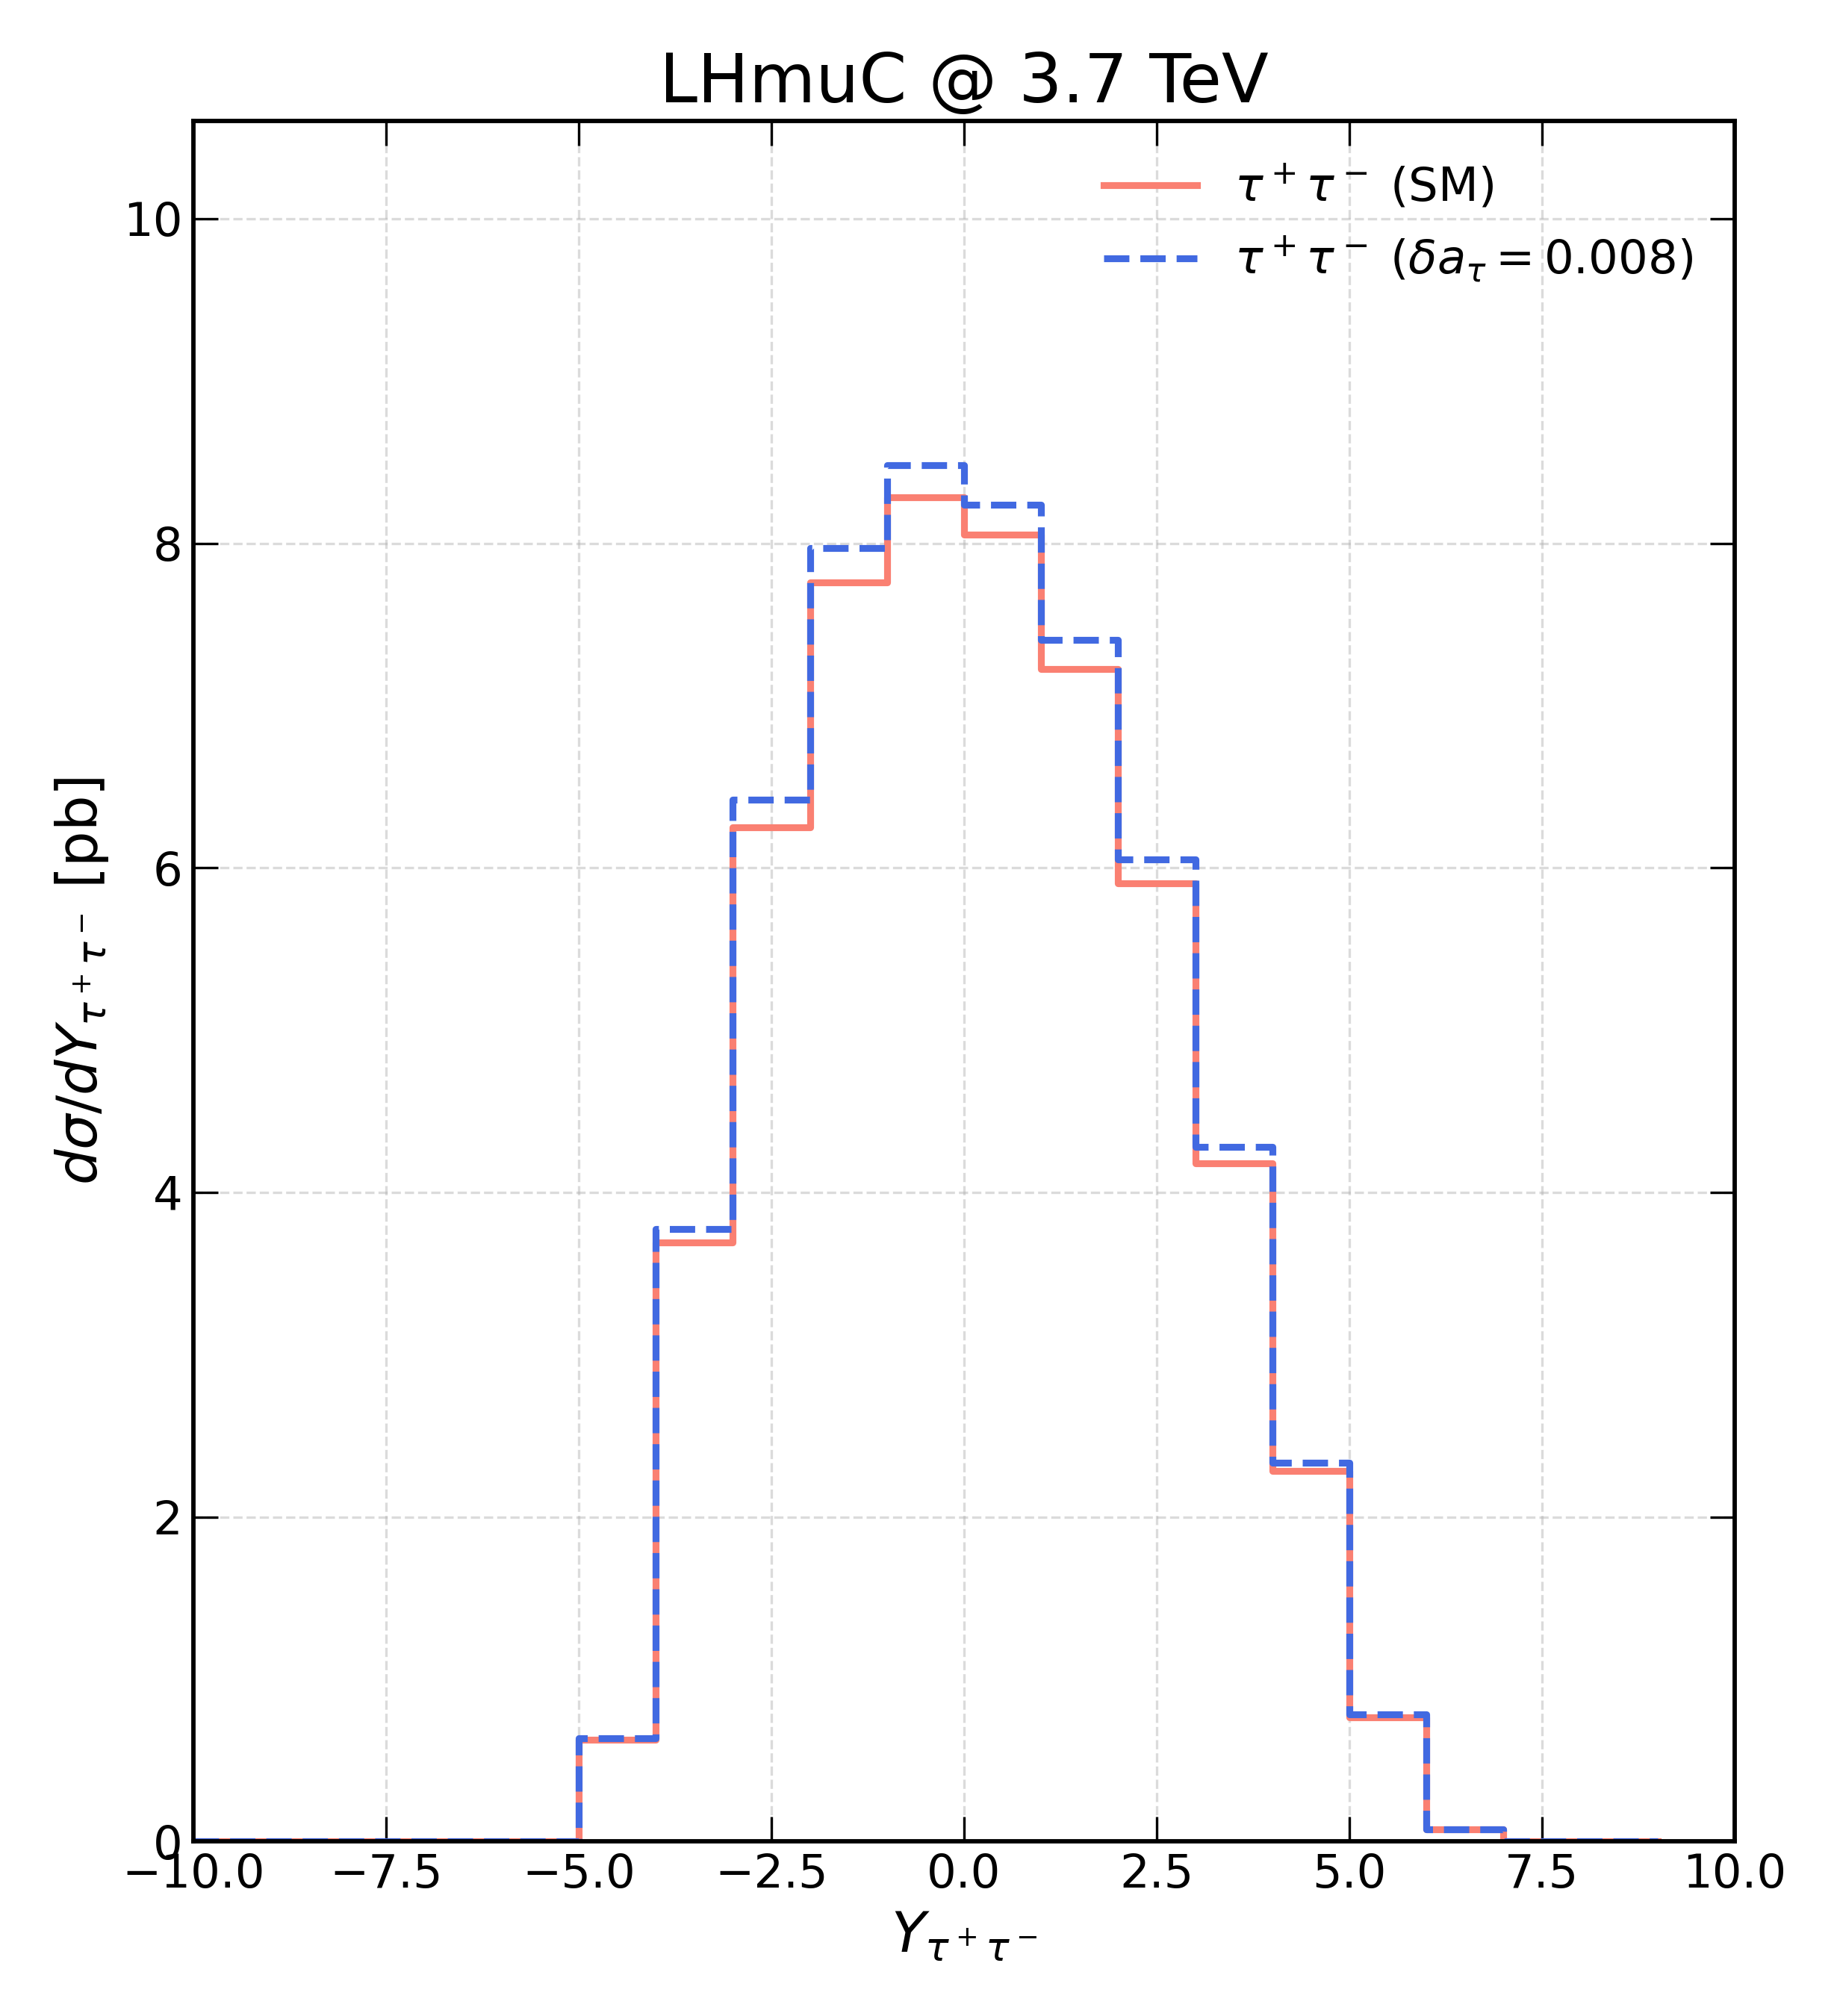
\includegraphics[width=\linewidth]{Rapidity_tau_pair_SM_vs_BSM_delta_aTau_LHmuC.png}
\end{column}
\end{columns}
\vspace{0.4em}
\begin{itemize}
\justifying
\small
%\item The rapidity distributions remain broadly central and are modified only mildly by the benchmark BSM coupling.
\item The \(\mathrm{LH}\mu\mathrm{C}\) distribution is more central because its \(p\mu^+\) beam-energy configuration is less asymmetric than the \(pe\) setup of the LHeC. As a result, the \(\gamma\gamma\) system has a smaller longitudinal boost, and the \(\tau^+\tau^-\) pair is produced closer to \(Y_{\tau^+\tau^-}\simeq 0\).
%\item Compared with the mass spectrum, the rapidity variable is less discriminating for the anomalous magnetic-moment benchmark.
%\item This supports the strategy of emphasizing the invariant-mass tail as the main sensitivity channel.
\end{itemize}
%\takehome{
% \justifying Rapidity is useful as a consistency check, but the dominant information on \atau\ comes from the mass spectrum rather than from a dramatic reshaping of \(\Ytt\).}
\end{frame}
%=====================================================



%=====================================================
\begin{frame}{Weighted physical ratio: LHeC vs LH$\mu$C}
\begin{columns}[T,onlytextwidth]
\begin{column}{0.49\textwidth}
\centering
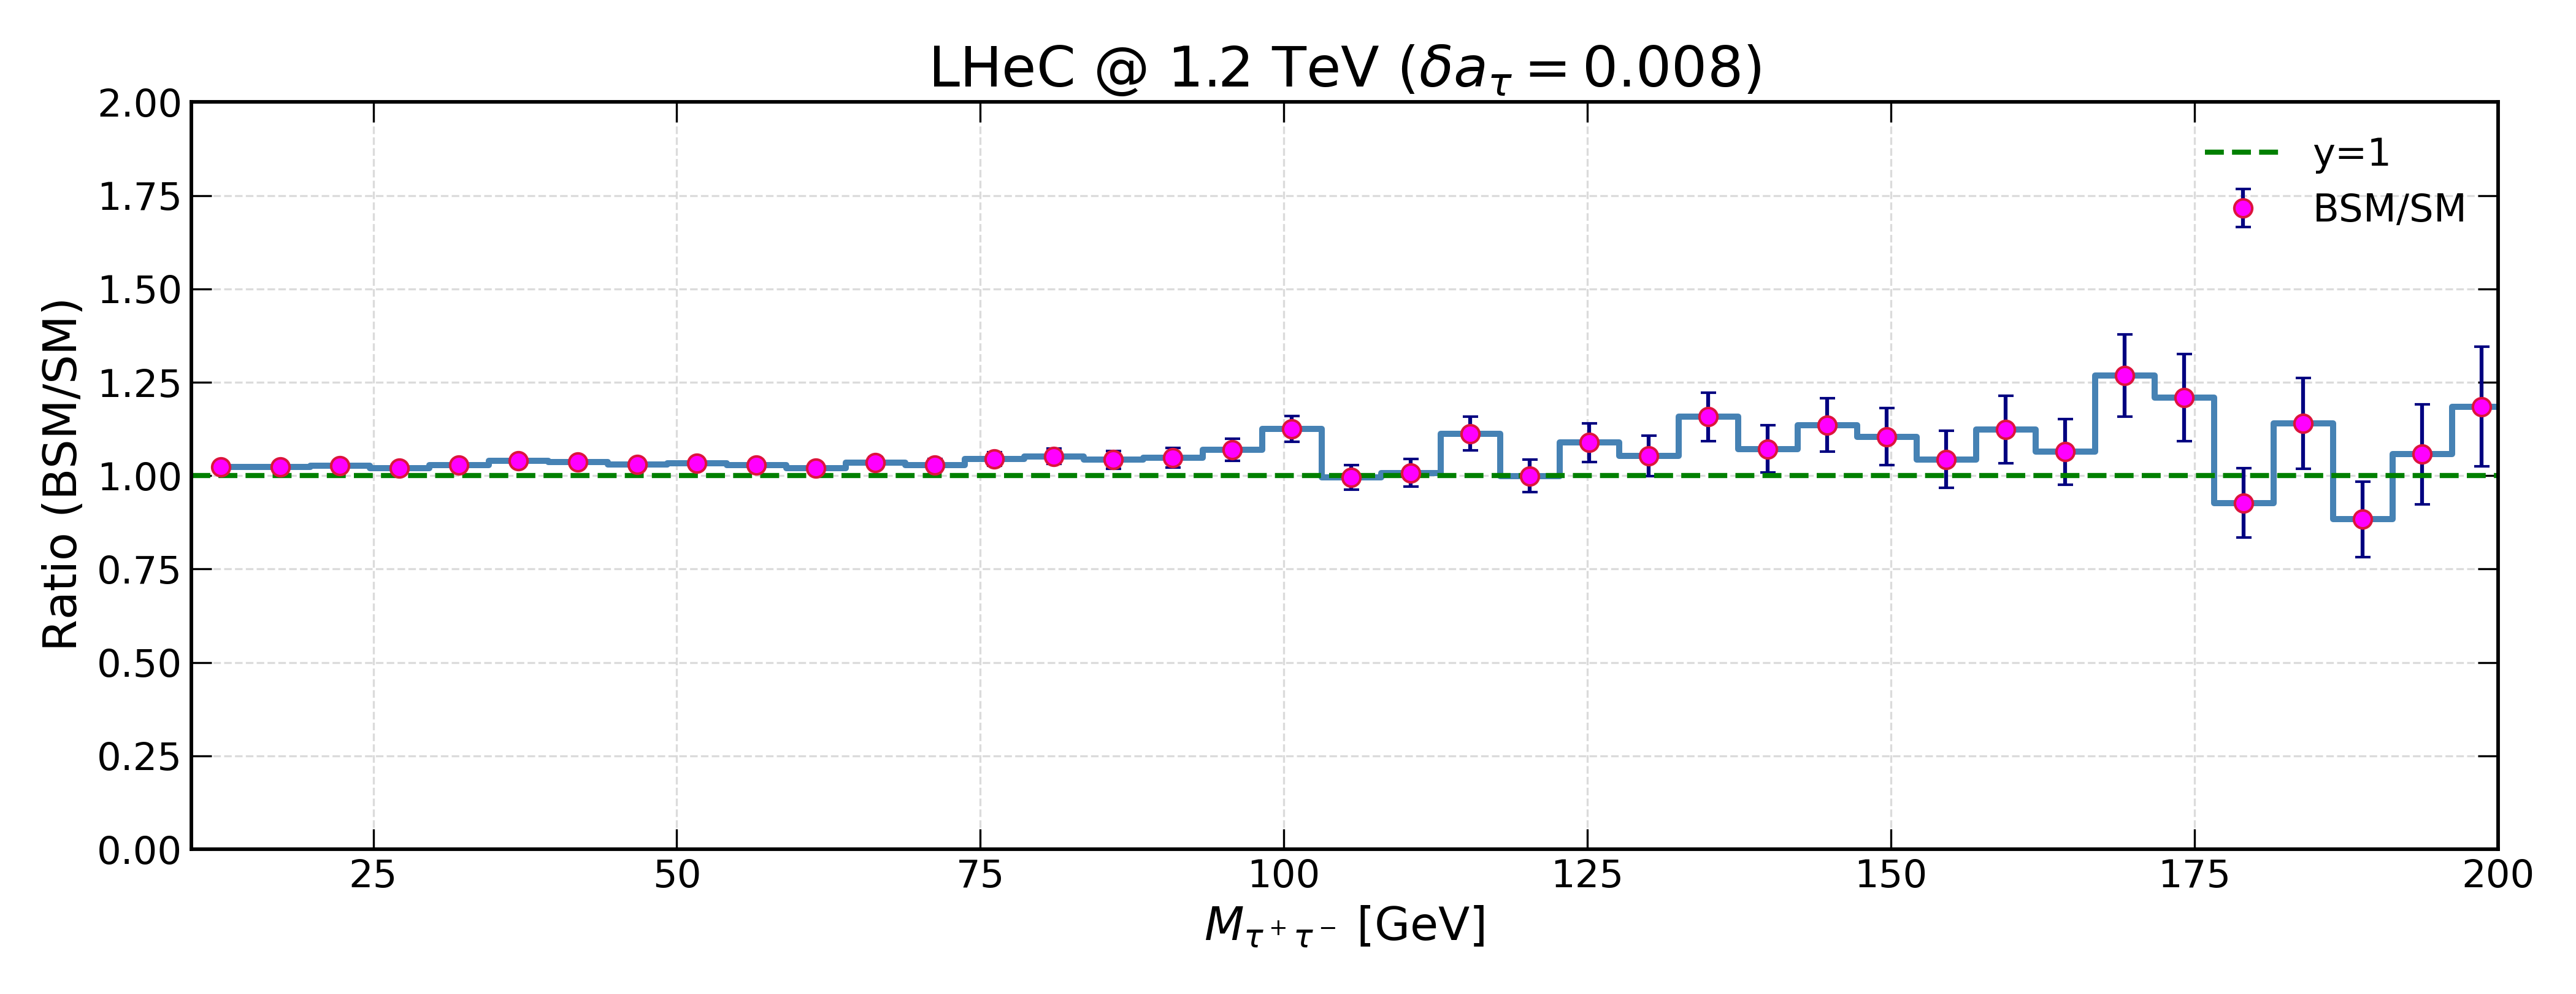
\includegraphics[width=\linewidth]{Ratio_BSM_over_SM_MtauTau_weighted_LHeC.png}
\end{column}
\begin{column}{0.49\textwidth}
\centering
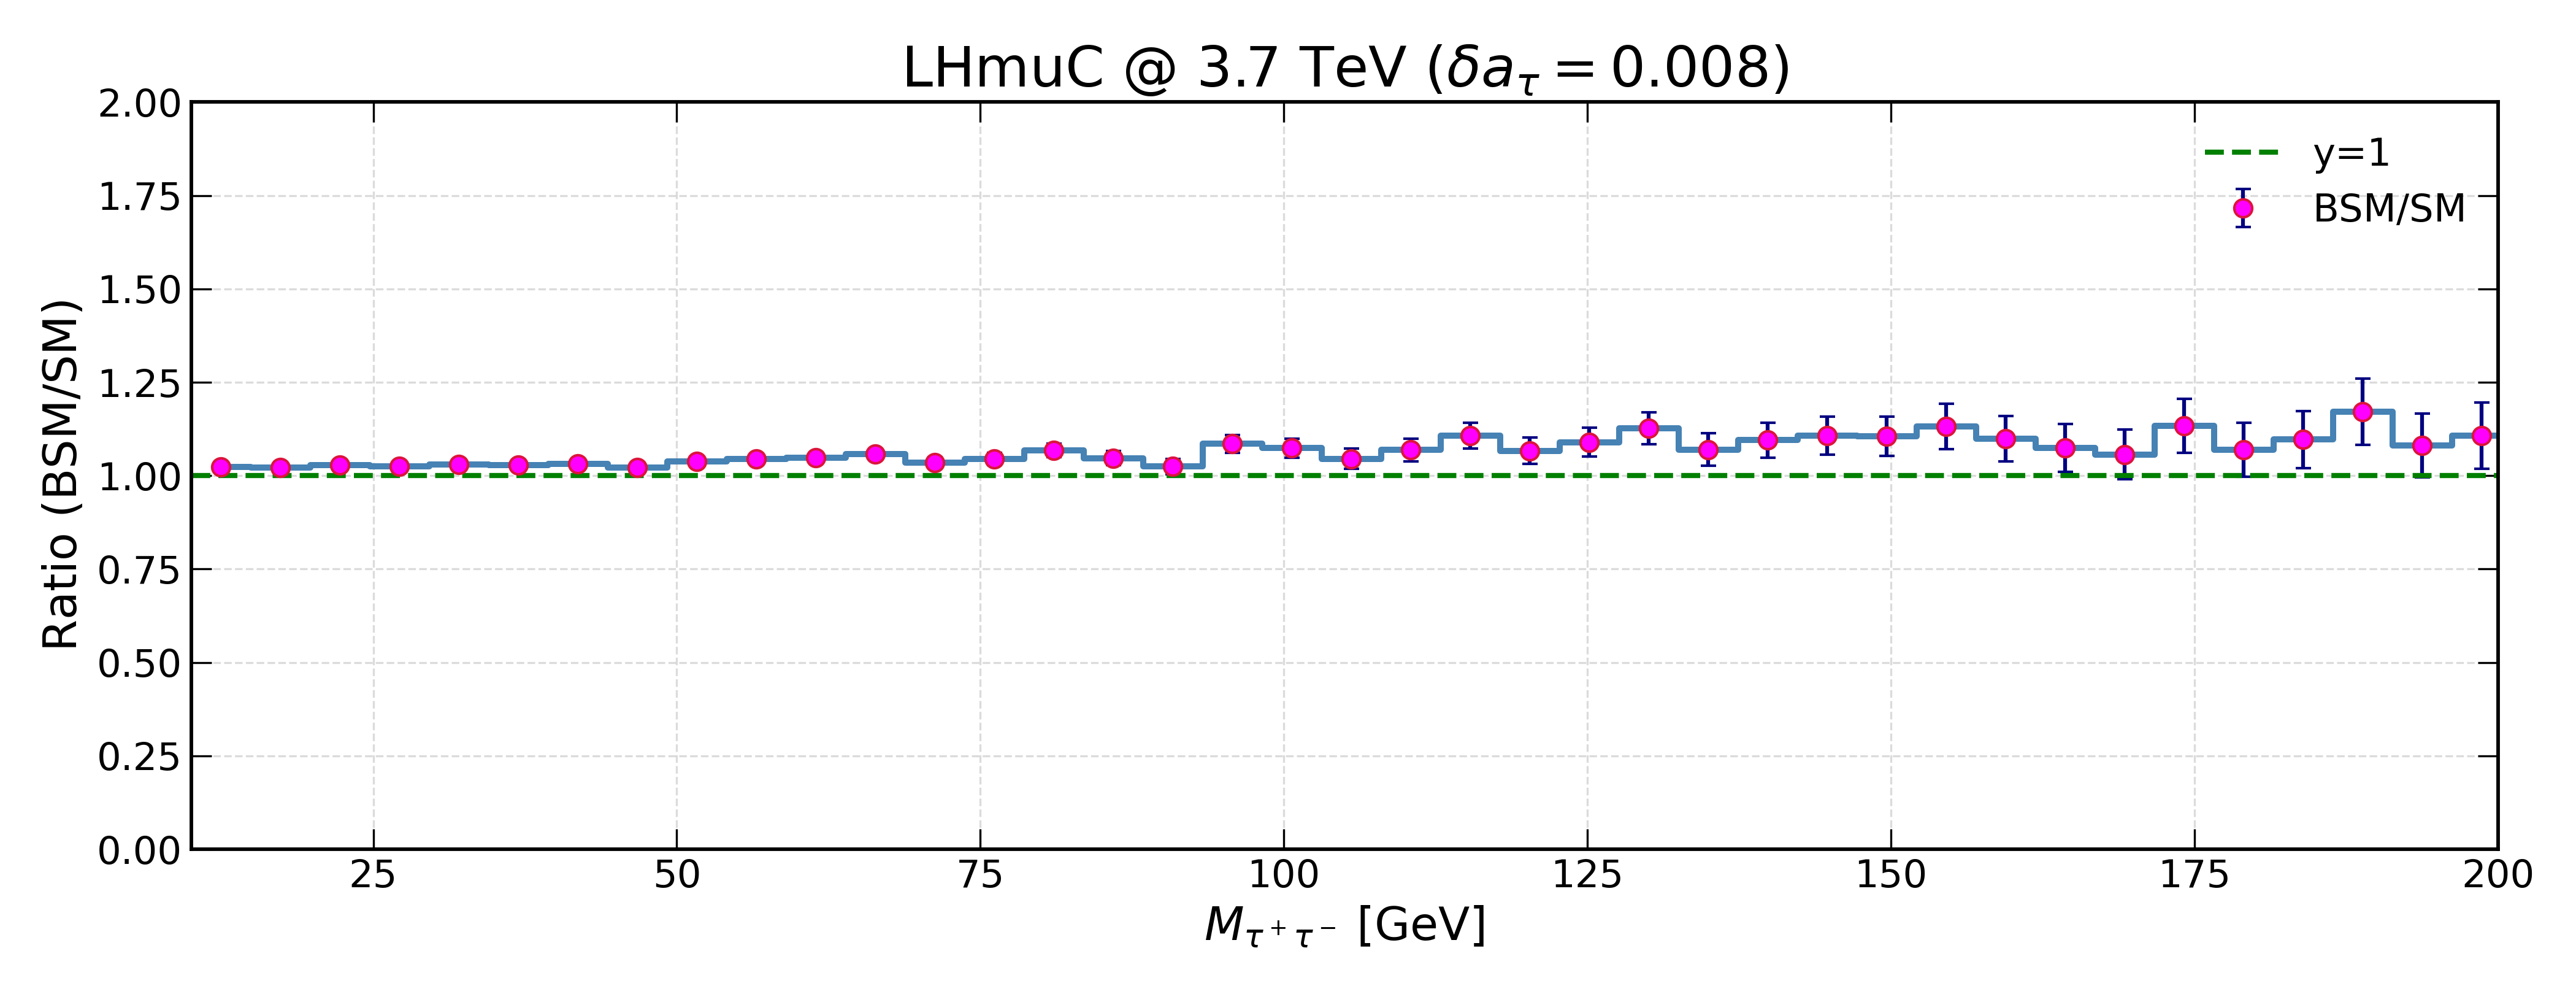
\includegraphics[width=\linewidth]{Ratio_BSM_over_SM_MtauTau_weighted_LHmuC.png}
\end{column}
\end{columns}
\vspace{0.4em}
\begin{itemize}
\justifying
\item This is the most directly physical comparison, because it uses the weighted differential spectra rather than only raw count ratios.
\item For both colliders, the ratio stays close to unity at low mass and rises above unity as the invariant mass increases.
\item The rise is stronger for the LH$\mu$C, showing that the same benchmark \(\datau\) produces a larger relative deviation from the SM in that environment.
\end{itemize}
\takehome{
\justifying
The physical ratio confirms the stronger high-mass BSM/SM deformation at the LH$\mu$C.}
\end{frame}
%=====================================================



%=====================================================
\begin{frame}{Uniform-bin linear-fit comparison}
\begin{columns}[T,onlytextwidth]
\begin{column}{0.49\textwidth}
\centering
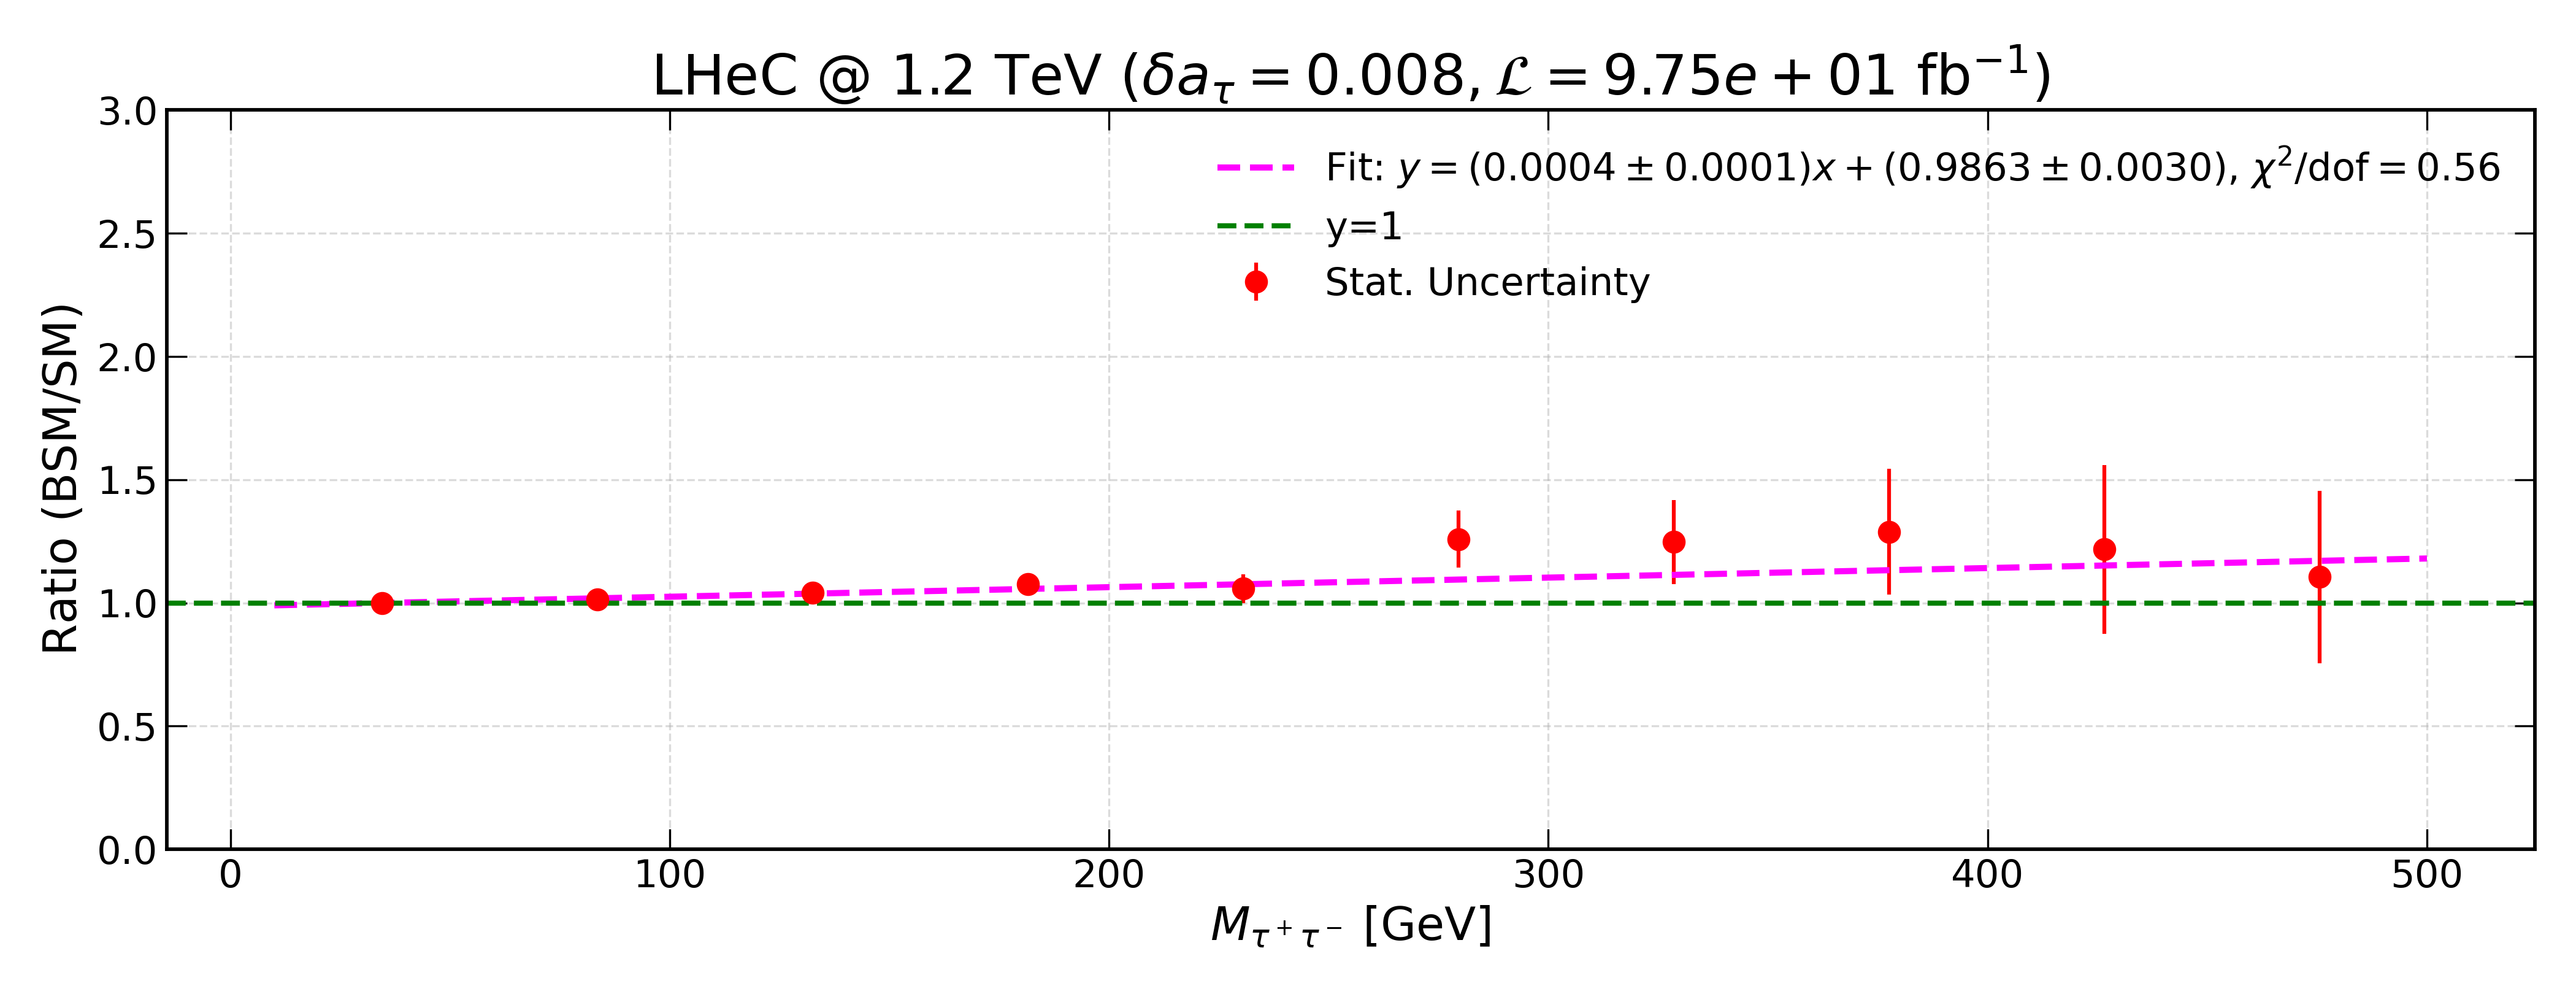
\includegraphics[width=\linewidth]{Ratio_Obs_Exp_with_Luminosity_Fit_uniform_LHeC.png}
\end{column}
\begin{column}{0.49\textwidth}
\centering
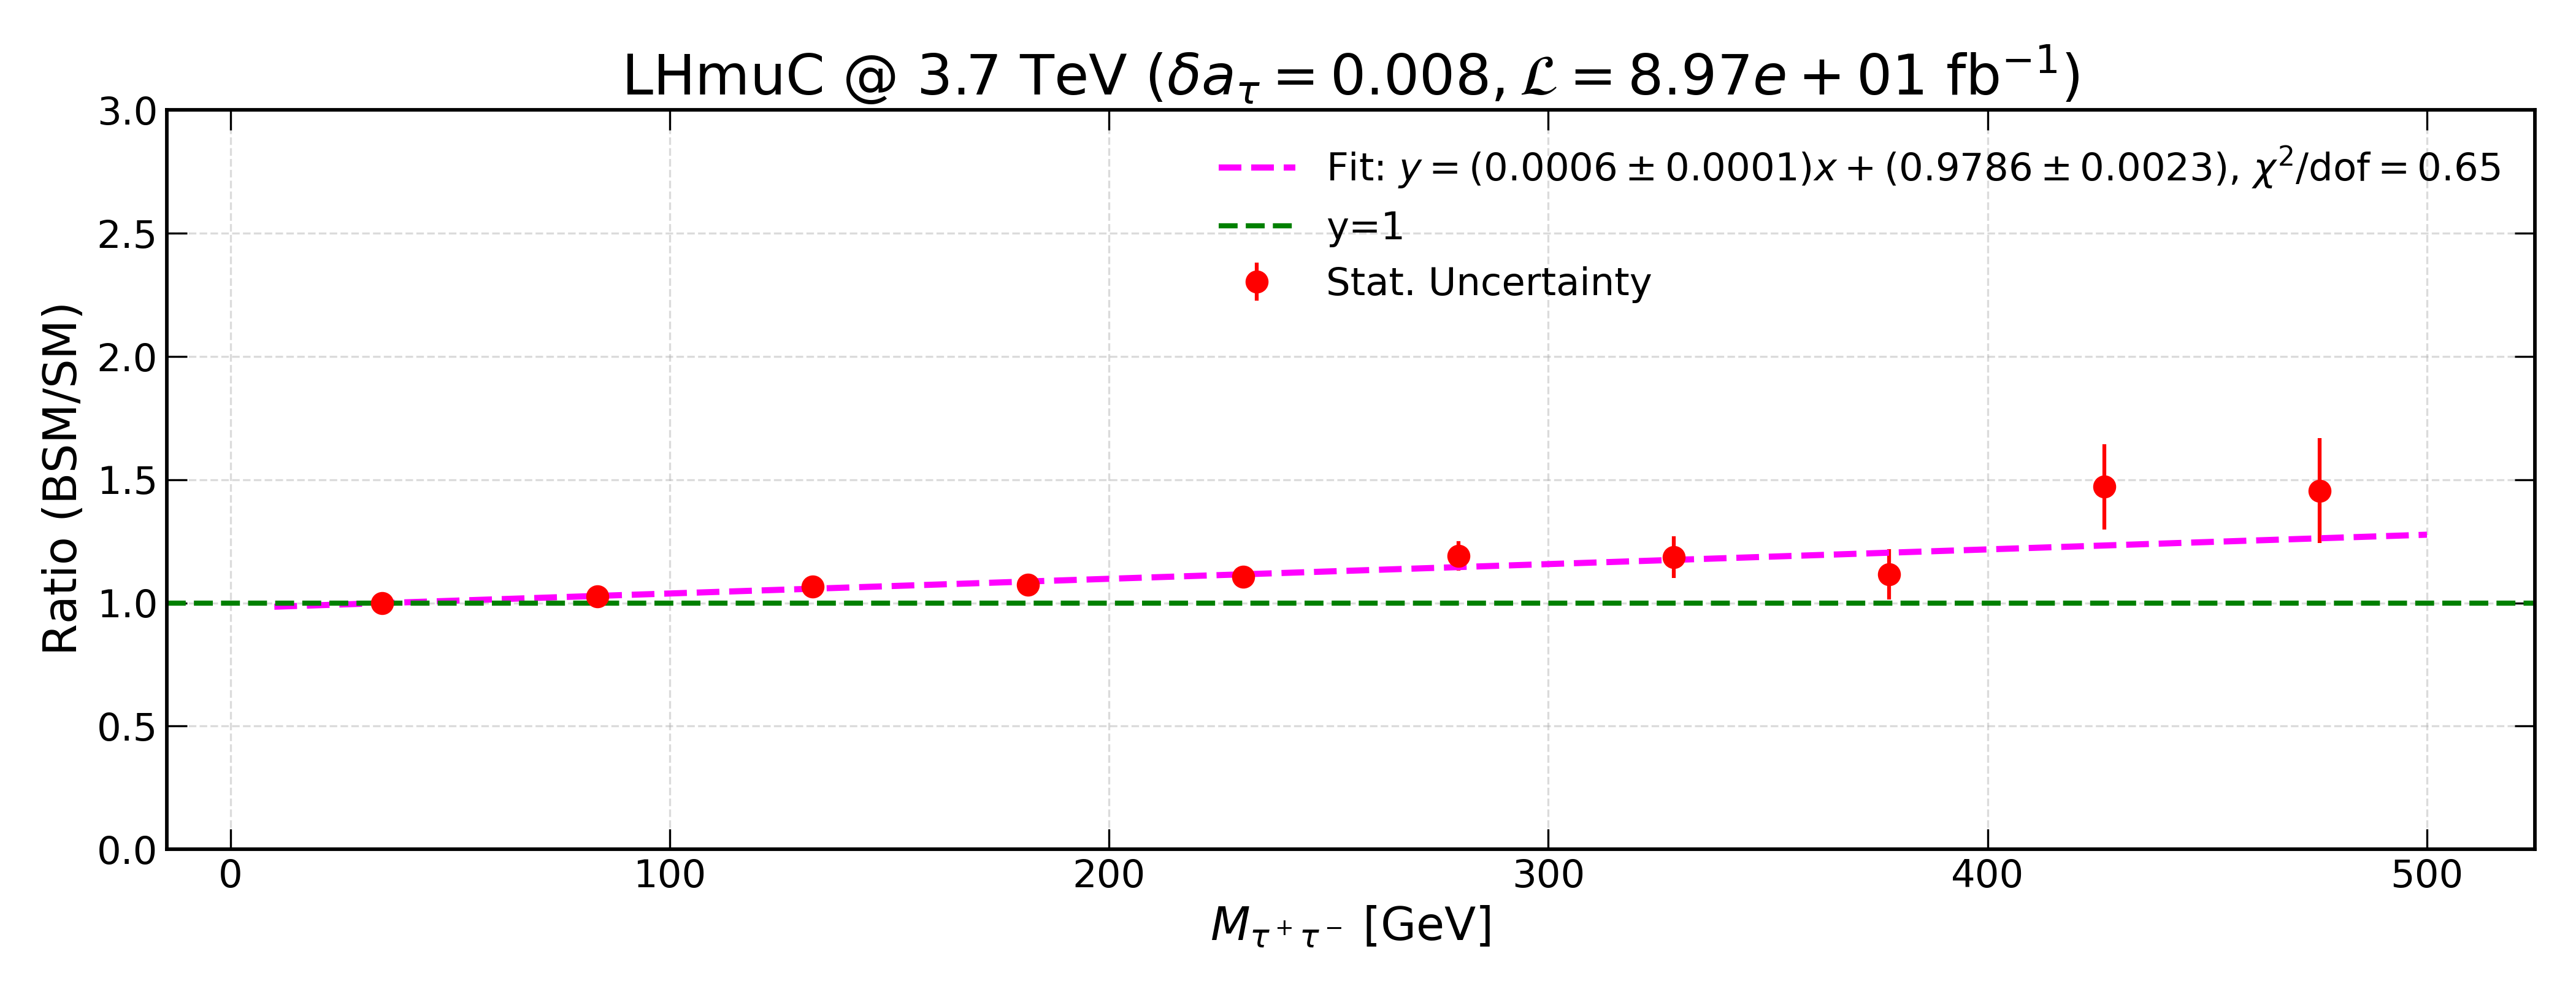
\includegraphics[width=\linewidth]{Ratio_Obs_Exp_with_Luminosity_Fit_uniform_LHmuC.png}
\end{column}
\end{columns}
\vspace{0.4em}
\begin{itemize}
\justifying
\item The linear fit \(y(M)=aM+b\) compresses the visual trend into a compact measure of tail hardening.
\item In the present benchmark study, the fitted slope is larger for the LH$\mu$C than for the LHeC.
\item A larger positive slope means a more rapidly growing departure from the SM toward high invariant mass.
\end{itemize}
\takehome{
\justifying Even at the level of a compact slope summary, the LH$\mu$C shows the stronger \atau-sensitive growth with \(\Mtt\).}
\end{frame}
%=====================================================


%=====================================================
\begin{frame}{Custom-bin linear-fit comparison}
\begin{columns}[T,onlytextwidth]
\begin{column}{0.49\textwidth}
\centering
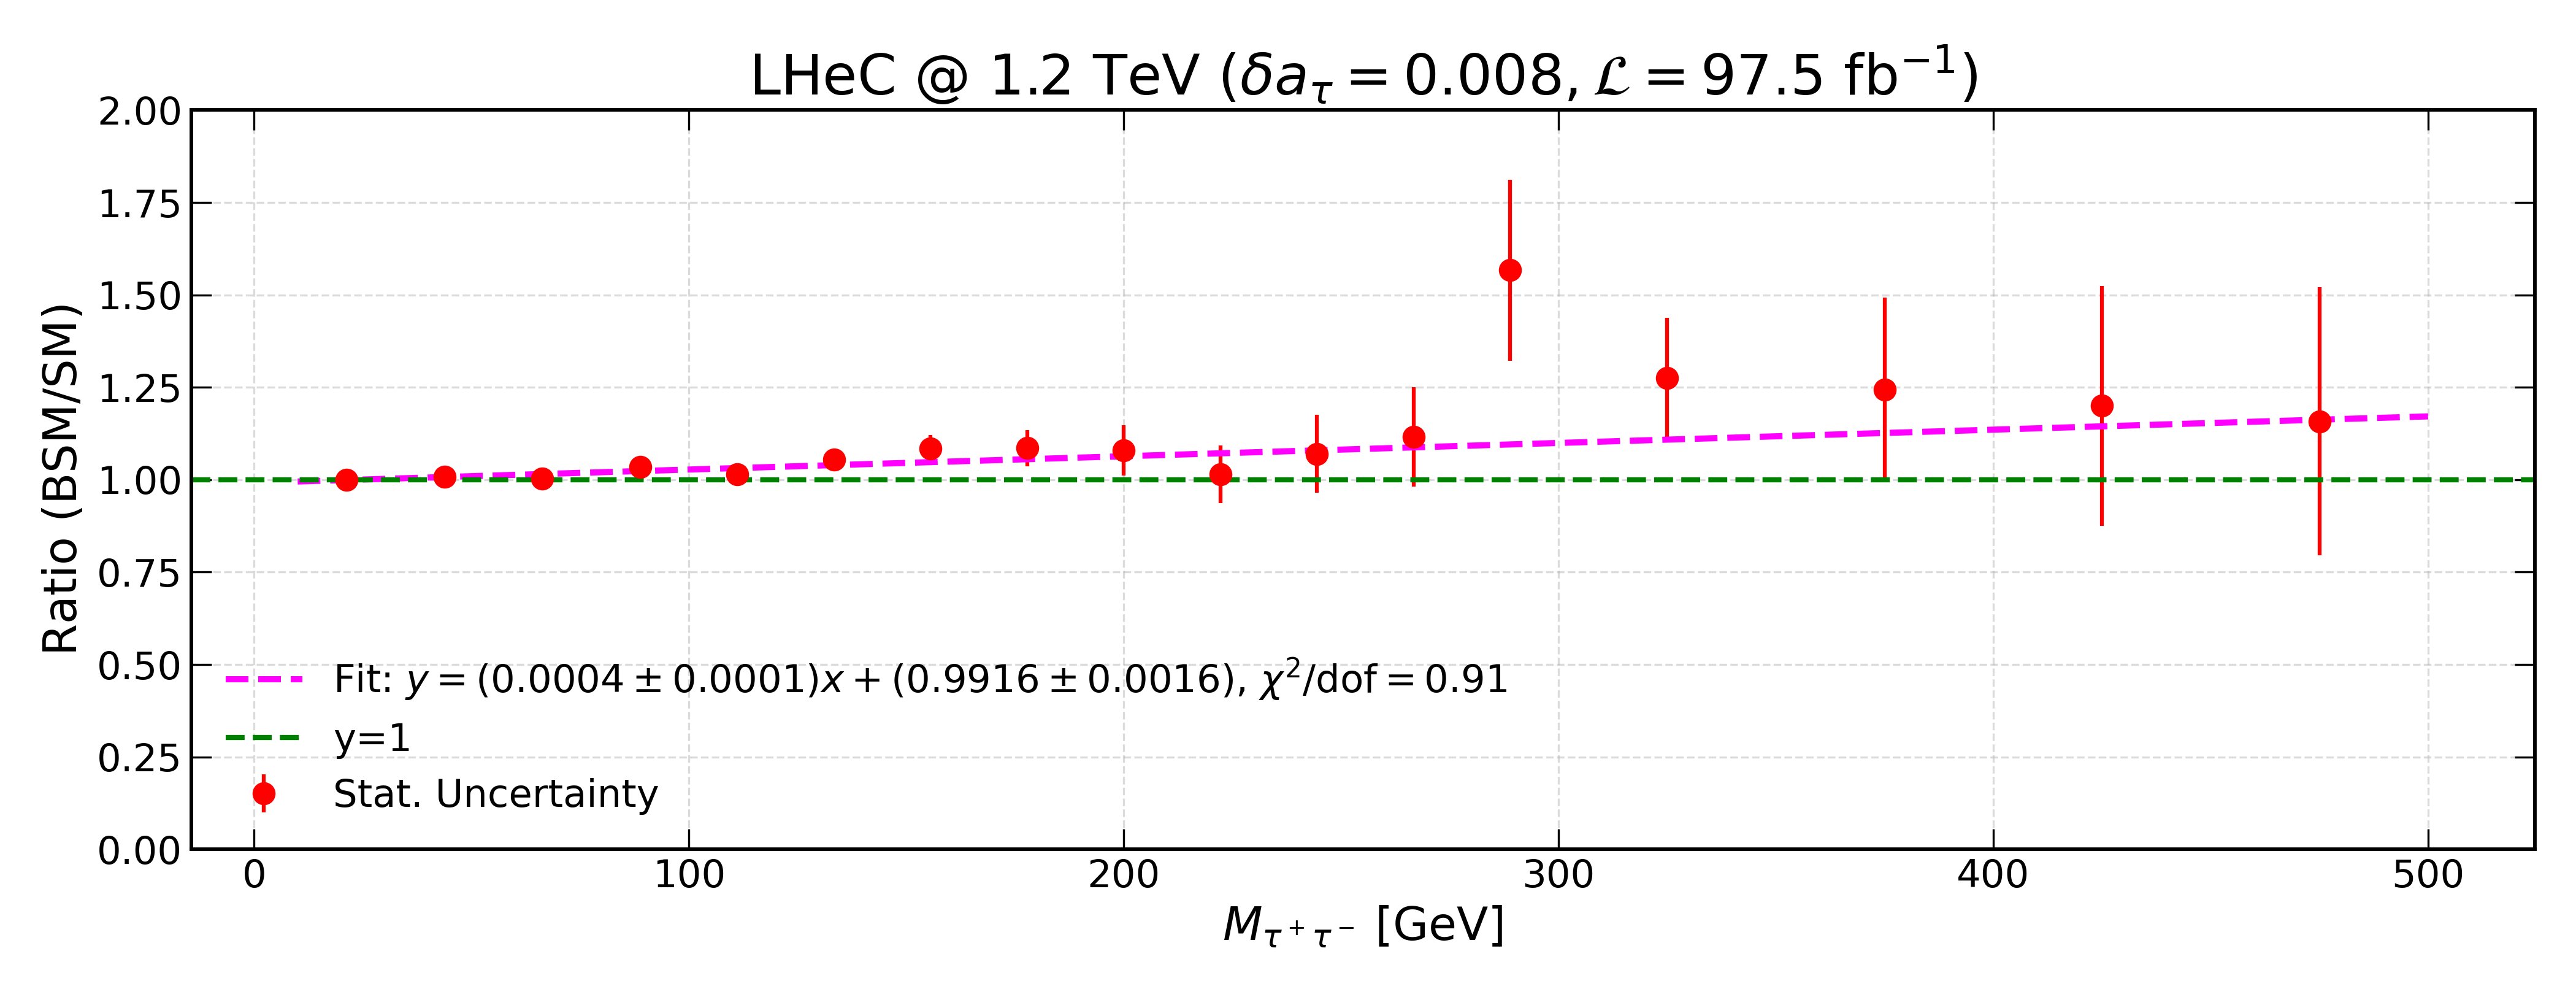
\includegraphics[width=\linewidth]{Ratio_Obs_Exp_with_Luminosity_Fit_custom_bins_LHeC.png}
\end{column}
\begin{column}{0.49\textwidth}
\centering
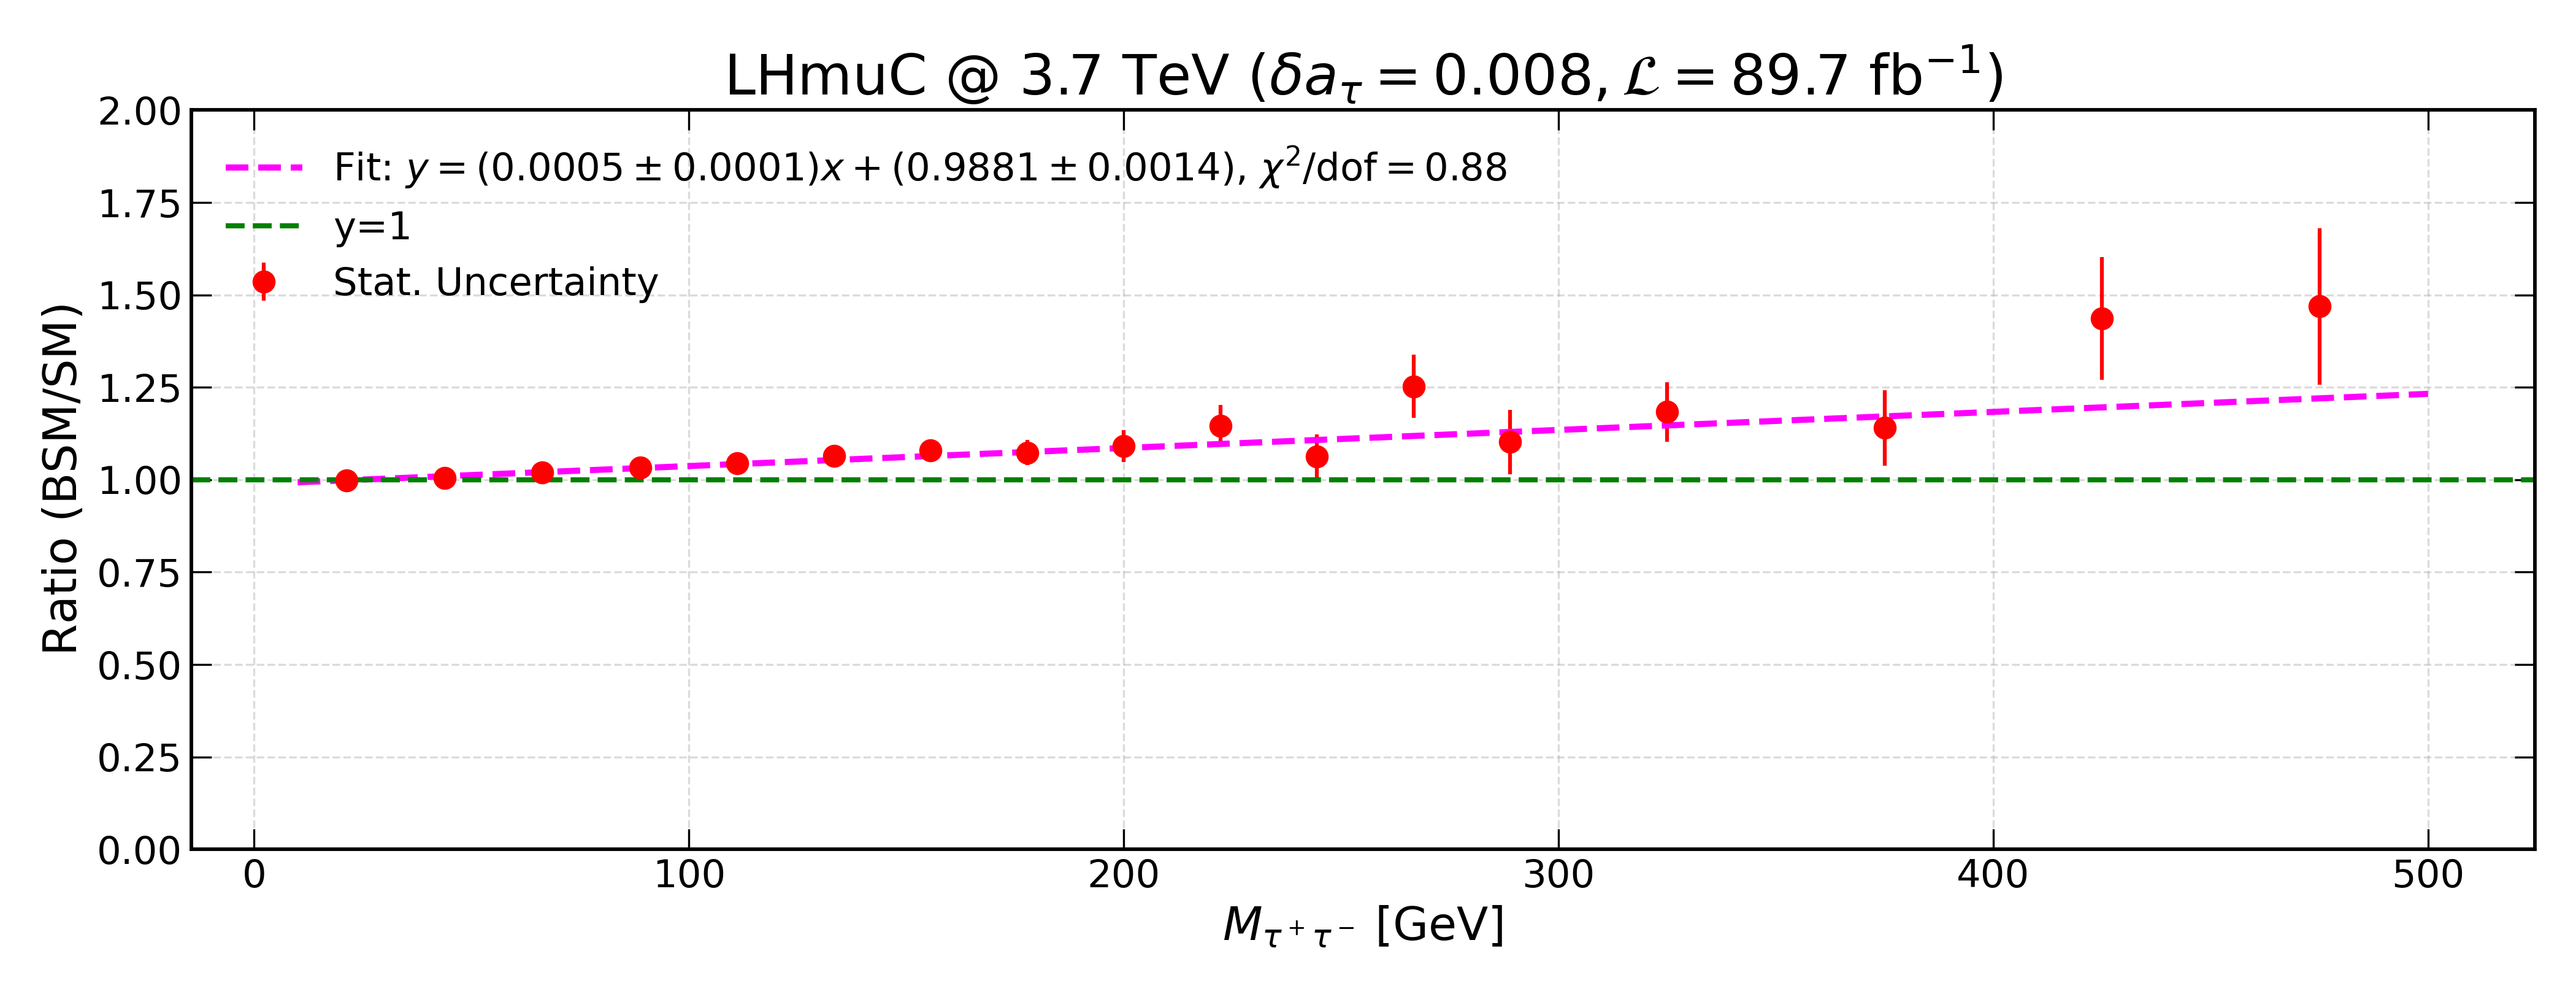
\includegraphics[width=\linewidth]{Ratio_Obs_Exp_with_Luminosity_Fit_custom_bins_LHmuC.png}
\end{column}
\end{columns}
\vspace{0.4em}
\begin{itemize}
\justifying
\item The custom-bin fit places more flexibility in the higher-mass region where the anomalous effect is most relevant.
\item The qualitative conclusion remains stable: the LH$\mu$C exhibits the steeper rise and therefore the stronger BSM sensitivity.
\item The hierarchy between colliders is therefore robust across the direct spectrum plots, weighted ratios, and the two fit strategies.
\end{itemize}
\takehome{
\justifying Across all comparison views in this benchmark study, the LH$\mu$C appears more sensitive to \atau\ than the LHeC.}
\end{frame}
%=====================================================



%=====================================================
\begin{frame}{Combined interpretation of the LHeC vs LH$\mu$C comparison}
\begin{columns}[T]
\begin{column}{0.53\textwidth}
\begin{block}{What all five comparisons consistently show}
\begin{itemize}
\justifying
\item The anomalous benchmark hardens the \(\tau^+\tau^-\) invariant-mass spectrum.
\item The rapidity spectrum changes much less strongly.
\item The BSM/SM ratio grows with \(\Mtt\) rather than remaining flat.
\item The growth is stronger for the LH$\mu$C than for the LHeC.
\end{itemize}
\end{block}
\end{column}
\begin{column}{0.45\textwidth}
\begin{exampleblock}{Scientifically careful conclusion}
\justifying
\small Within the present \textbf{truth-level benchmark study} based on merged MadGraph LHE samples, the LH$\mu$C appears more promising than the LHeC for probing \atau\ through photon-induced \(\tau^+\tau^-\) production.
\end{exampleblock}
\end{column}
\end{columns}
\vspace{0.5cm}
\begin{itemize}
\justifying
\item This statement concerns the current generator-level setup and should not yet be read as a final detector-level exclusion result.
\end{itemize}
\end{frame}
%=====================================================



\section{Current CMS Context and Future-Collider Motivation}


%=====================================================
\begin{frame}{How the future-collider study connects to CMS pp results}
\begin{columns}[T]
\begin{column}{0.63\textwidth}
\begin{itemize}
\justifying
\item CMS has observed \(\gamma\gamma\to\tau^+\tau^-\) in pp collisions and used the rate and mass-shape information to constrain \atau\ and \dtau.
\item The analysis relies on an exclusivity strategy: low hadronic activity, low acoplanarity, and low track multiplicity near the dilepton or ditau vertex.
\item The key conceptual overlap with our future-collider study is the same: BSM effects are enhanced in the higher-mass region.
\item Future lepton--hadron colliders offer a complementary environment in which photon-induced processes can be studied with different beam kinematics and cleaner initial-state control.
\end{itemize}
\end{column}
\begin{column}{0.55\textwidth}
\begin{figure}
\centering
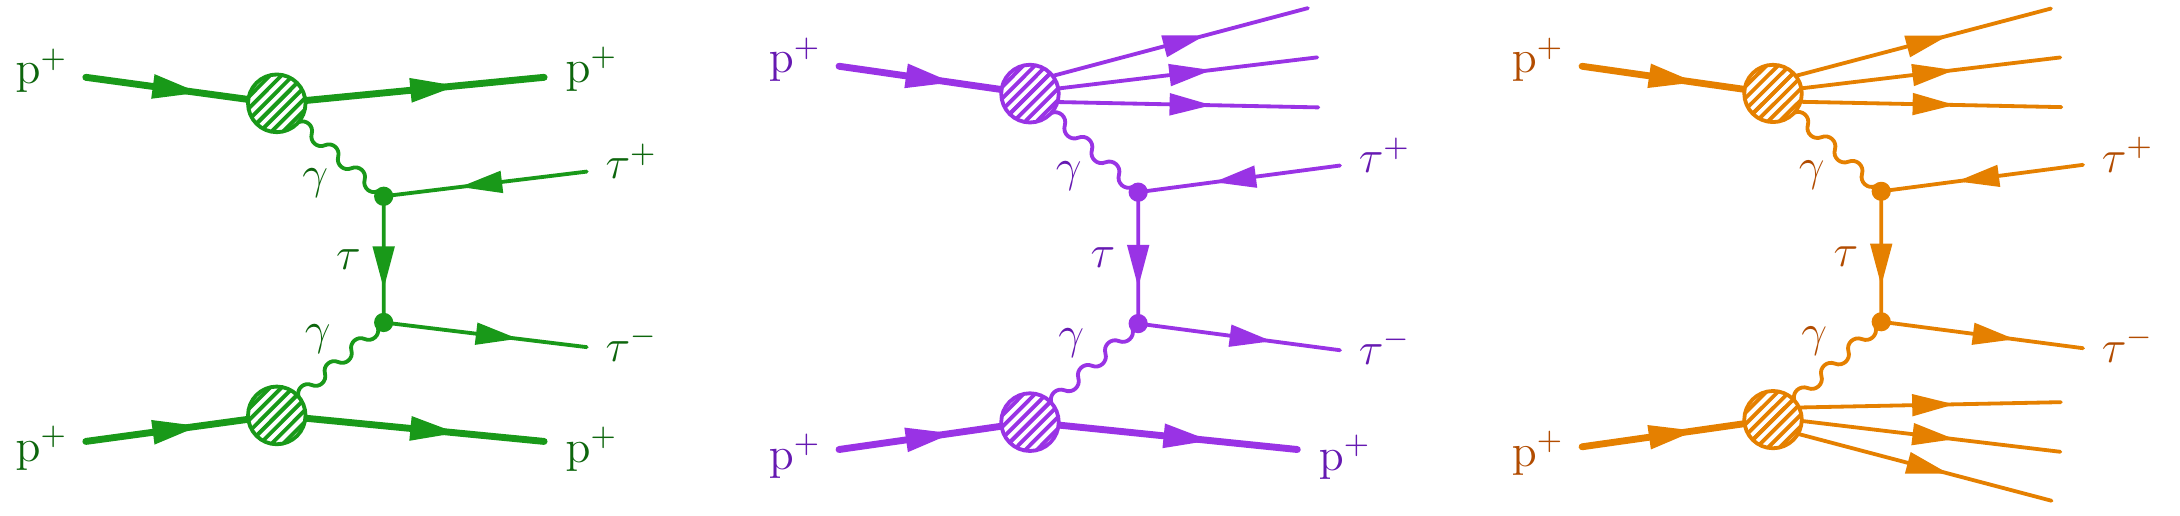
\includegraphics[width=\linewidth]{pptautau_CMS.png}
\caption{\small
\justifying
Schematic illustration of photon-induced \(\gamma\gamma \to \tau^+\tau^-\) production in \(pp\) collisions, showing the elastic, semiexclusive, and dissociative topologies relevant for the CMS analysis. }
\end{figure}
\end{column}
\end{columns}
\end{frame}
%=====================================================





\section{Conclusions and Outlook}


%=====================================================
\begin{frame}{Main conclusions}
\begin{itemize}
\justifying
\item We studied photon-induced \(\gamma\gamma\to\tau^+\tau^-\) production at two future lepton--hadron colliders: the {\color{red}LHeC} and the {\color{blue}LH$\mu$C}.
\item The benchmark anomalous coupling \(\datau=0.008\) hardens the invariant-mass spectrum relative to the Standard Model.
\item The rapidity distributions are comparatively less discriminating than the mass spectrum.
\item The BSM/SM ratio grows with \(\Mtt\), showing that the hard tail is the key region for sensitivity.
\item Across the invariant-mass, weighted-ratio, and fit-based comparisons, the {\color{blue}LH$\mu$C} exhibits the stronger high-mass response.
\end{itemize}
\begin{alertblock}{Bottom line}
\justifying
\small In the present truth-level benchmark study, the {\color{blue}{LH$\mu$C}} is favored over the {\color{red}LHeC} for probing the anomalous magnetic moment \atau\ in photon-induced $\tau$-pair production.
\end{alertblock}
\end{frame}
%=====================================================



%=====================================================
\begin{frame}{Outlook}
\begin{itemize}
\justifying
\item Extend the study from truth level to realistic detector-level analyses.
\item Implement acceptance and reconstruction effects for the relevant visible $\tau$ final states.
\item Translate the present shape distortions into explicit projected constraints on \atau.
\item Generalize the benchmark study to the CP-odd sector and to simultaneous fits in the \((\ctb,\ctw)\) plane.
\item Explore luminosity scenarios, optimization of mass-window selections, and systematic uncertainties.
\item Connect the future-collider projections more directly to the CMS pp strategy and other current measurements.
\end{itemize}
\end{frame}
%=====================================================








%=====================================================
\begin{frame}[plain,noframenumbering]
\centering
\includegraphics[width=\paperwidth,height=\paperheight,keepaspectratio]{Thank_You.jpg}
\end{frame}
%=====================================================




\appendix
\section*{Backup}


%=====================================================
\begin{frame}[fragile]{Backup: MG settings summary}
\begin{block}{Hard-process setup}
\scriptsize\ttfamily
import model SMEFTsim\_top\_alphaScheme\_UFO\\
generate a a > ta+ ta- / h h1 NP=0 SMHLOOP=0\\
\vspace{0.5ex}
import model SMEFTsim\_top\_alphaScheme\_UFO\\
generate a a > ta+ ta- / h h1 NP<=2 SMHLOOP=0
\end{block}
\begin{itemize}
\centering
    \item Beam configurations: \(7~\mathrm{TeV}\oplus 50~\mathrm{GeV}\) for LHeC and \(7~\mathrm{TeV}\oplus 500~\mathrm{GeV}\) for LH$\mu$C.
    \item Equivalent-photon setup through \texttt{iww}; minimal generation cut \(m_{\ell\ell}>10~\mathrm{GeV}\).
\end{itemize}
\end{frame}
%=====================================================


%=====================================================
\begin{frame}{Backup: EFT parameter summary}
\centering
\begin{tabular}{>{\raggedright\arraybackslash}p{0.30\textwidth}p{0.60\textwidth}}
\toprule
Quantity & Role in the study \\
\midrule
\textcolor{TauBlue}{\(\atau,\ \datau\)} & CP-even anomalous magnetic-moment sector \\
\textcolor{TauGreen}{\(\dtau,\ \ddtau\)} & CP-odd electric-dipole sector \\
\textcolor{TauOrange}{\(\ctb,\ctw\)} & SMEFT Wilson coefficients entering the tau dipole interaction \\
\textcolor{TauOrange}{\(\Lam\)} & EFT scale used for normalization of the dim-6 operators \\
\(\Mtt\) & primary sensitivity observable in the present benchmark study \\
\bottomrule
\end{tabular}
\end{frame}
%=====================================================


%=====================================================
\begin{frame}{Backup: sample statistics summary}
\centering
\begin{tabular}{>{\raggedright\arraybackslash}p{0.26\textwidth}cccc}
\toprule
Collider & $N_{\mathrm{runs}}$ & $N_{\mathrm{evts/run}}$ & $N_{\mathrm{tot}}$ & $\mathcal{L}_{\mathrm{eff}}$ [fb$^{-1}$] \\
\midrule
LHeC SM / BSM & 5 & $10^6$ & $5\times10^6$ & $\sim 97.5$ \\
LH$\mu$C SM / BSM & 5 & $10^6$ & $5\times10^6$ & $\sim 89.7$ \\
\bottomrule
\end{tabular}
\vspace{1em}
\begin{itemize}
 \justifying
    \item Cross sections are read from the LHE headers and combined with event-count weighting.
    \item The effective luminosities summarize the sample sizes used by the plotting and fitting workflow.
\end{itemize}
\end{frame}
%=====================================================



%=====================================================
\begin{frame}{Backup: side-by-side weighted-ratio comparison}
\begin{columns}[T,onlytextwidth]
\begin{column}{0.49\textwidth}
\centering
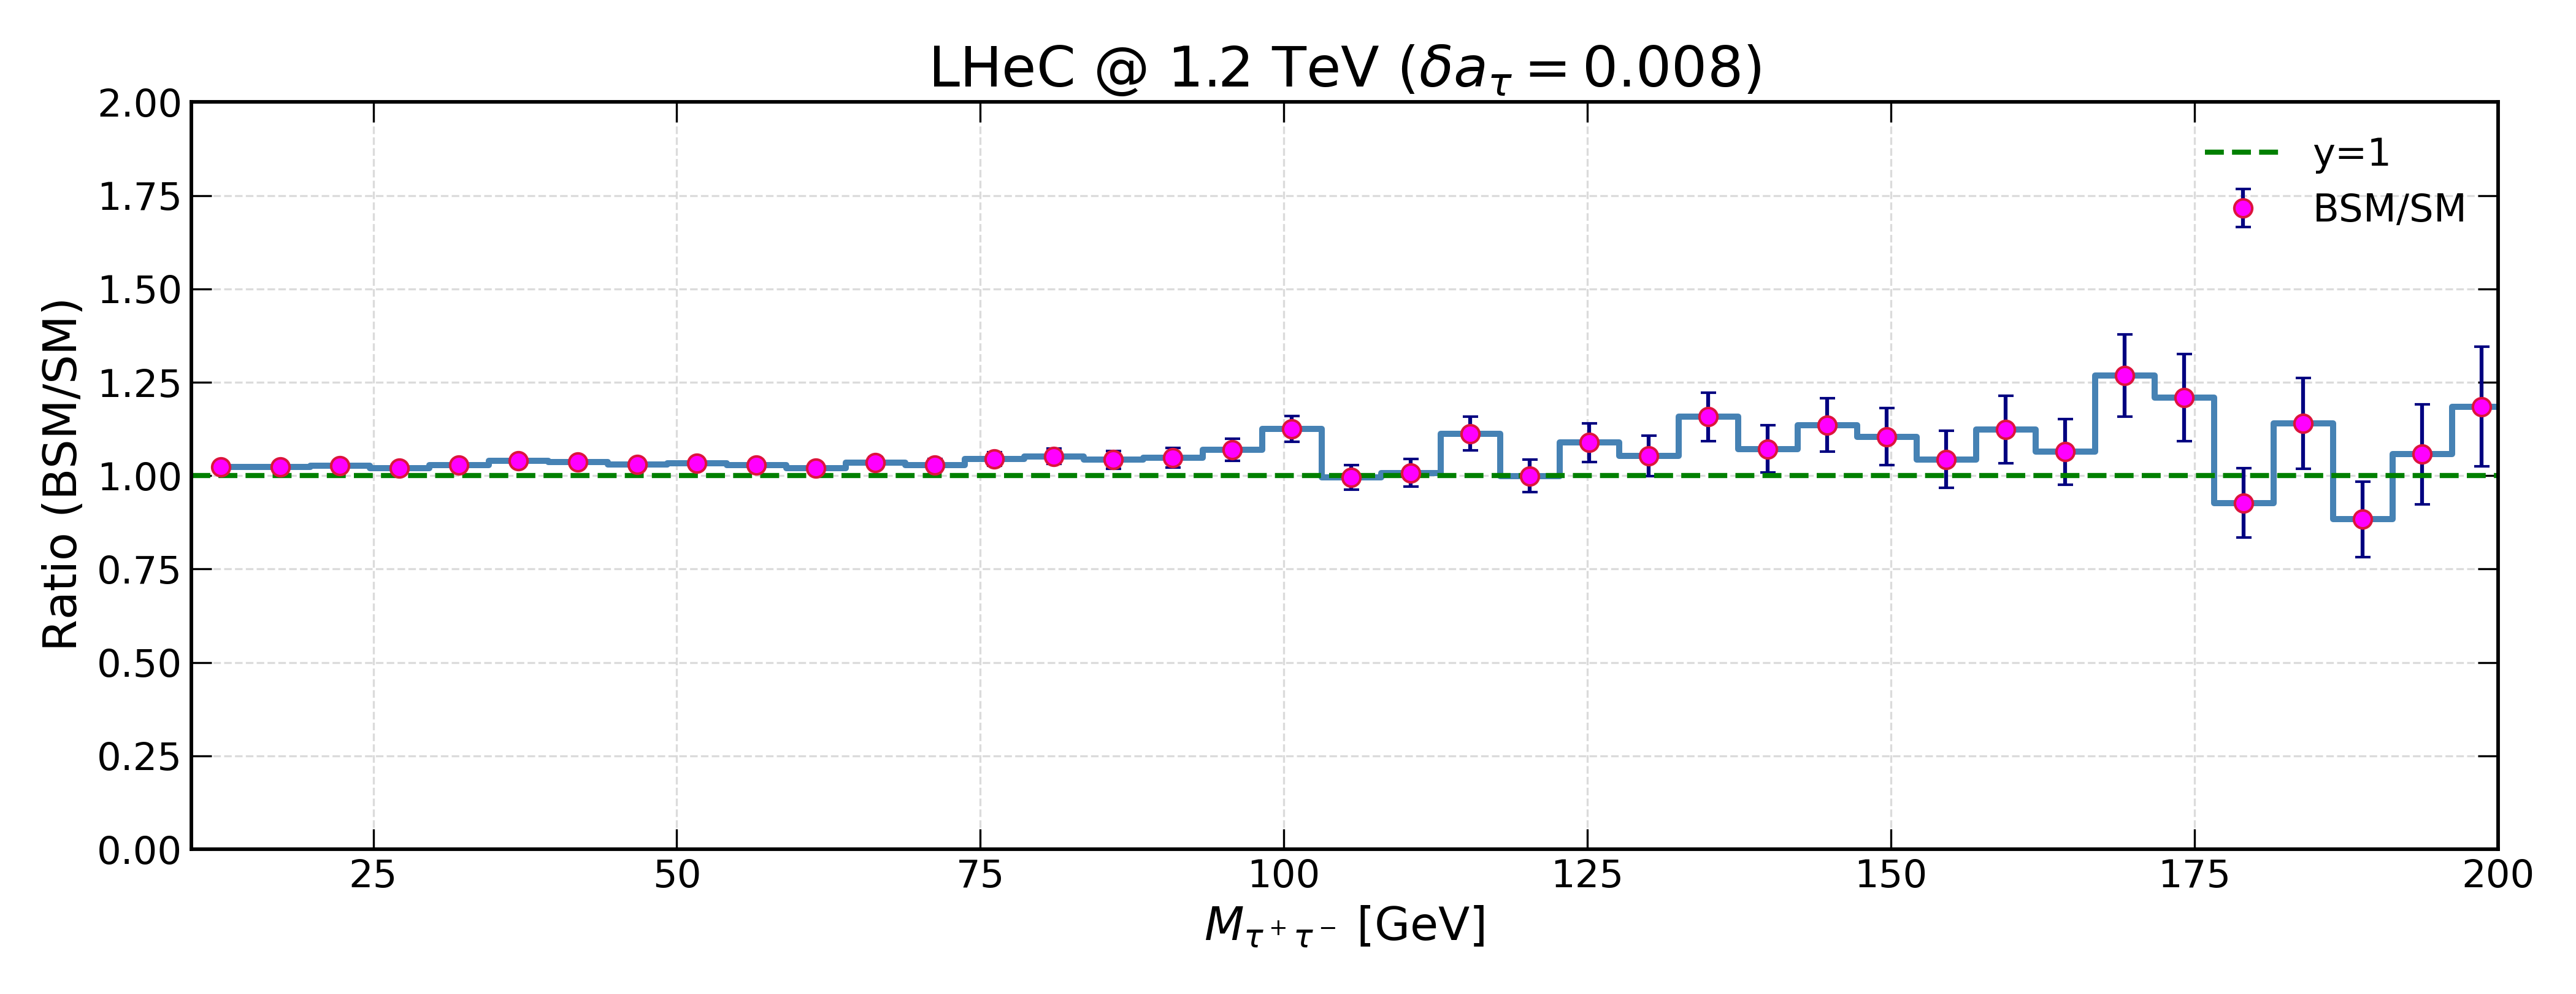
\includegraphics[width=\linewidth]{Ratio_BSM_over_SM_MtauTau_weighted_LHeC.png}
\end{column}
\begin{column}{0.49\textwidth}
\centering
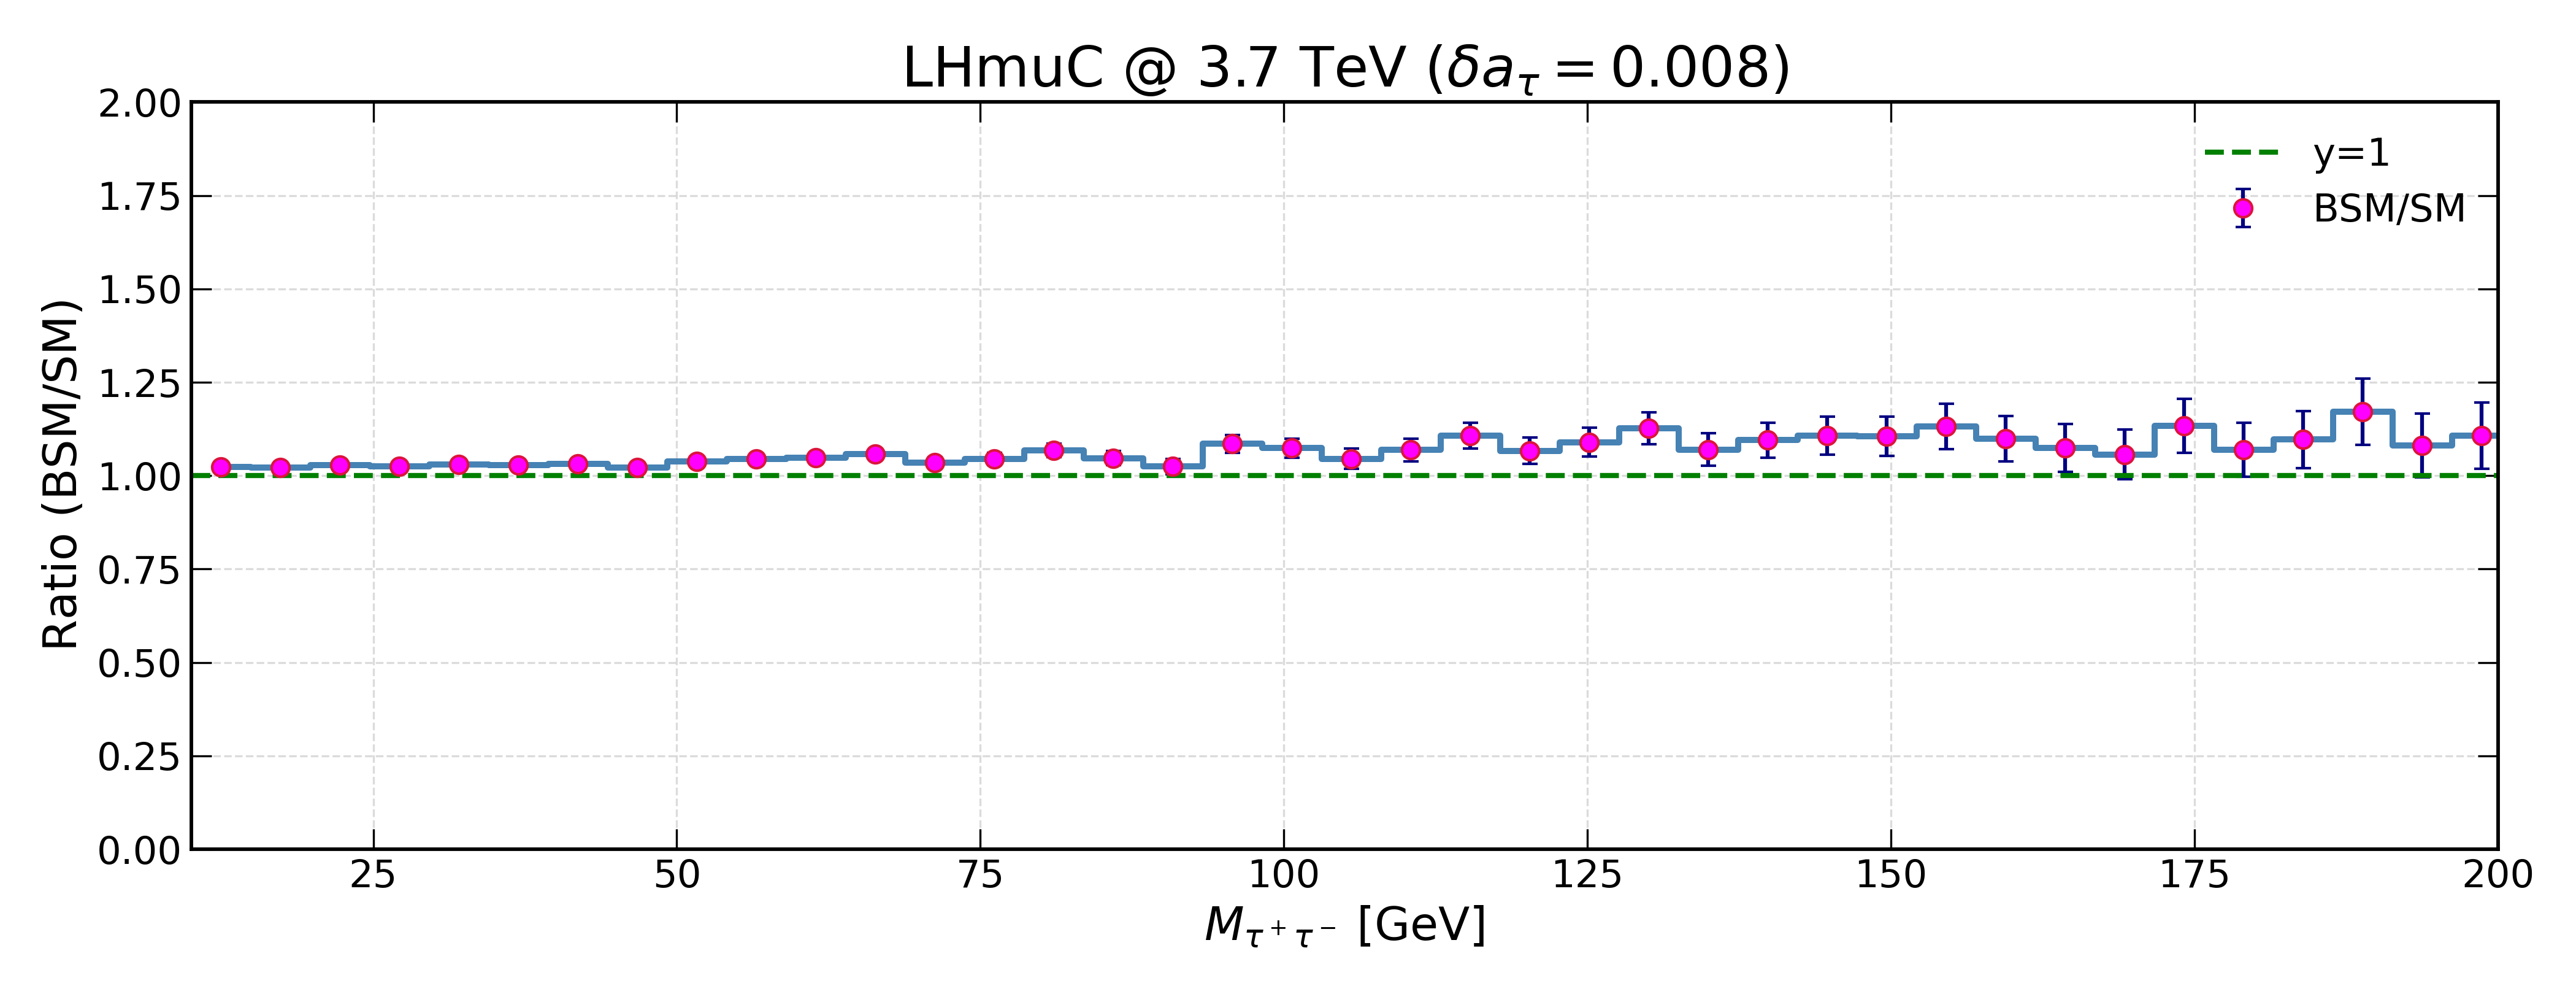
\includegraphics[width=\linewidth]{Ratio_BSM_over_SM_MtauTau_weighted_LHmuC.png}
\end{column}
\end{columns}
\vspace{0.5em}
\takehome{The weighted BSM/SM ratio remains the clearest visual summary of why the LH$\mu$C appears more sensitive to \atau\ in this benchmark study.}
\end{frame}
%=====================================================


\end{document}

%=====================================================



%=====================================================
\begin{frame}{CMS-inspired observables and why the hard tail matters}
	\begin{columns}[T]
		\begin{column}{0.48\textwidth}
			% 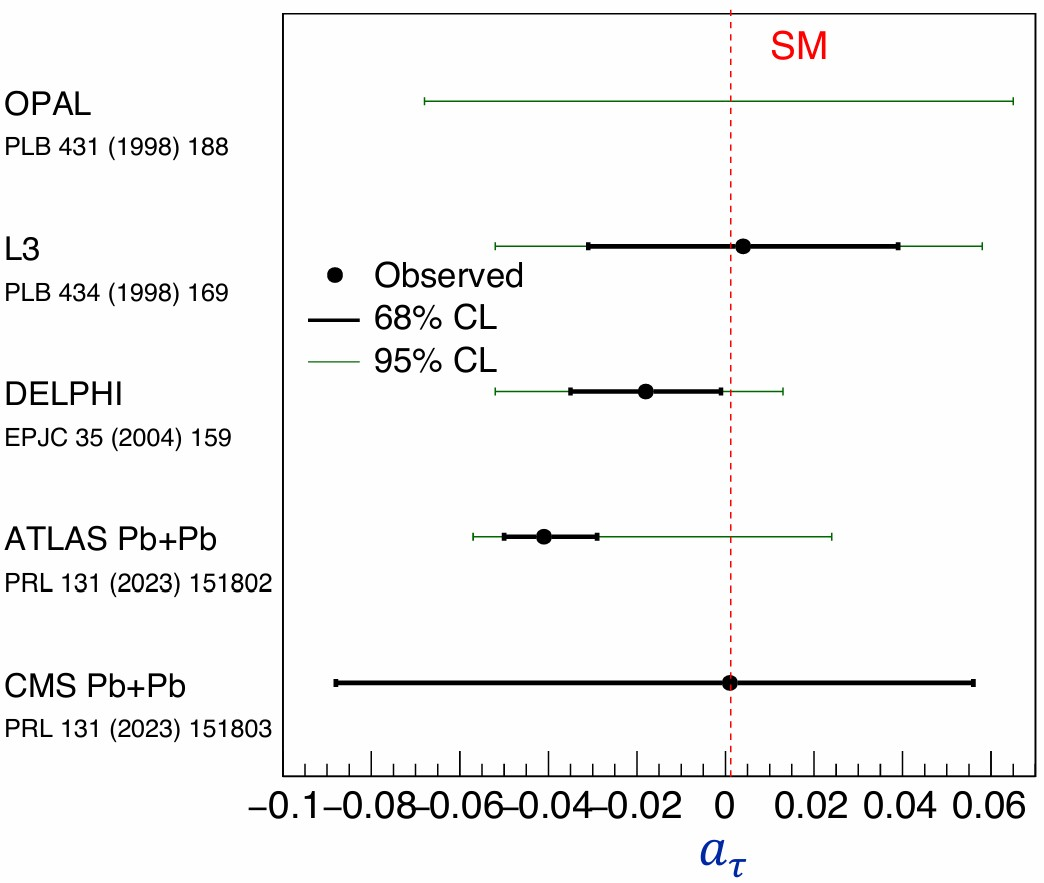
\includegraphics[width=\linewidth]{cms_world_aTau_dTau.png}
			% TODO: add world-comparison screenshot
			\placeholdergraphic{World status figure for \(\atau\) and \(\dtau\).}{0.44\textheight}
		\end{column}
		\begin{column}{0.48\textwidth}
			% \includegraphics[width=\linewidth]{cms_likelihood_aTau.png}
			% TODO: add likelihood scan screenshot
			\placeholdergraphic{Likelihood scan or confidence-interval figure for \(\atau\).}{0.44\textheight}
		\end{column}
	\end{columns}
	\vspace{0.5em}
	\begin{itemize}
		\justifying
		\item In CMS, the accessible phase space and the exclusivity strategy make the mass shape central for BSM sensitivity.
		\item The future LHeC/LH$\mu$C study follows the same general logic at truth level: the hard region carries the most visible anomalous-coupling information.
	\end{itemize}
\end{frame}
%=====================================================



%=====================================================
\begin{frame}{CMS control-region and exclusivity placeholders}
	\begin{columns}[T]
		\begin{column}{0.48\textwidth}
			% \includegraphics[width=\linewidth]{cms_ntracks_validation.png}
			% TODO: add screenshot of Ntracks validation / low-track excess
			\placeholdergraphic{Track-multiplicity validation / low-track signal-region motivation.}{0.44\textheight}
		\end{column}
		\begin{column}{0.48\textwidth}
			% \includegraphics[width=\linewidth]{cms_mumu_control_region.png}
			% TODO: add screenshot of mu mu control region / elastic rescaling figure
			\placeholdergraphic{Muon control-region figure for dissociative rescaling / elastic normalization.}{0.44\textheight}
		\end{column}
	\end{columns}
	\vspace{0.5em}
	\begin{itemize}
		\justifying
		\item These CMS ingredients are useful reference points for the long-term detector-level development of the lepton--hadron collider study.
		\item They motivate how future work can move beyond truth-level shapes toward realistic sensitivity projections.
	\end{itemize}
\end{frame}
%=====================================================\\



